\ifdefined\isphone
  \documentclass[a6paper,11pt,oneside]{book}

\usepackage{algpseudocode}
\usepackage{algorithm}
\usepackage{amsfonts}
\usepackage{amsmath,amsthm,amssymb}
\usepackage{graphicx}
\usepackage{hyperref}
\usepackage{mathtools}
\usepackage{steinmetz}
\usepackage{fancyvrb}
\usepackage{textcomp}
\usepackage{gensymb}
\usepackage[normalem]{ulem}
\usepackage[T1]{fontenc}
\usepackage{cmap}
\usepackage{xspace}

\DeclareGraphicsExtensions{.pdf,.png,.jpg}

\newcommand{\mb}[1]{\ensuremath{\mathbb{{#1}}}}
\newcommand{\setof}[1]{\ensuremath{\left \{ #1 \right \}}}
\newcommand{\tuple}[1]{\ensuremath{\left \langle #1 \right \rangle }}

\DeclarePairedDelimiter{\ceil}{\lceil}{\rceil}
\DeclarePairedDelimiter{\floor}{\lfloor}{\rfloor}

\DeclareSymbolFont{bbold}{U}{bbold}{m}{n}
\DeclareSymbolFontAlphabet{\mathbbold}{bbold}

\newtheorem{statement}{Statement}
\newtheorem{rmk}{Remark}
\newtheorem{defi}{Definition}
\newtheorem{example}{Example}
\newtheorem{theorem}{Theorem}
\newtheorem{lemma}[theorem]{Lemma}
\newtheorem{proposition}[theorem]{Proposition}
\newtheorem{pf}[theorem]{Proof}
\newtheorem{corollary}[theorem]{Corollary}

% Differences
\usepackage[margin=5mm]{geometry}
\usepackage{tgheros}
\renewcommand*\familydefault{\sfdefault}

\else
  \documentclass[11pt,oneside]{book}

\usepackage{algpseudocode}
\usepackage{algorithm}
\usepackage{amsfonts}
\usepackage{amsmath,amsthm,amssymb}
\usepackage{graphicx}
\usepackage{hyperref}
\usepackage{mathtools}
\usepackage{steinmetz}
\usepackage{fancyvrb}
\usepackage{textcomp}
\usepackage{gensymb}
\usepackage[normalem]{ulem}
\usepackage[T1]{fontenc}
\usepackage{cmap}
\usepackage{xspace}

\DeclareGraphicsExtensions{.pdf,.png,.jpg}

\newcommand{\mb}[1]{\ensuremath{\mathbb{{#1}}}}
\newcommand{\setof}[1]{\ensuremath{\left \{ #1 \right \}}}
\newcommand{\tuple}[1]{\ensuremath{\left \langle #1 \right \rangle }}

\DeclarePairedDelimiter{\ceil}{\lceil}{\rceil}
\DeclarePairedDelimiter{\floor}{\lfloor}{\rfloor}

\DeclareSymbolFont{bbold}{U}{bbold}{m}{n}
\DeclareSymbolFontAlphabet{\mathbbold}{bbold}

\newtheorem{statement}{Statement}
\newtheorem{rmk}{Remark}
\newtheorem{defi}{Definition}
\newtheorem{example}{Example}
\newtheorem{theorem}{Theorem}
\newtheorem{lemma}[theorem]{Lemma}
\newtheorem{proposition}[theorem]{Proposition}
\newtheorem{pf}[theorem]{Proof}
\newtheorem{corollary}[theorem]{Corollary}

% Differences
\setlength{\textheight}{9.5in}
\setlength{\textwidth}{7.0in}
\setlength{\topmargin}{-0.75in}
\setlength{\oddsidemargin}{-0.25in}
\setlength{\evensidemargin}{0.75in}
\setlength{\parskip}{0.15in}
\setlength{\parindent}{0in}

\fi
\begin{document}

\newcommand{\Sln}{\textbf{Solution.} }
\newcommand{\Lap}{$\Lapm$}
\newcommand{\Lapm}{\mathcal{L}}
\newcommand{\dy}{\dot{y}}
\newcommand{\dx}{\dot{x}}
\newcommand{\ddy}{\ddot{y}}
\newcommand{\ddx}{\ddot{x}}
\newcommand{\chpm}{characteristic polynomial}

\DefineShortVerb{\#}

%\vspace{-1.0in}
\begin{center}
\Large{SE 380 Winter 2013: Notes} \\
\end{center}



\hrulefill\

\hfill Shale Craig


\begin{enumerate}
    \item Control Engineering
        \begin{enumerate}
            \item Control engineering is creating control functions to regulate functions for known (and unknown) values.
            \item Systems are made up of plants and controllers.

                \begin{enumerate}
                    \item Plants are the system we want to change. They are an 3-tuple of, related by $g(t)$

                    \begin{enumerate}
                        \item Disturbance function: $d(t)$.
                        \item Reference function: $u(t)$ [Generally a heaviside function, which we use convolution to add up]
                        \item Output function: $y(t)$.
                    \end{enumerate}

                    \item Controllers are systems we use to change the plant. Specified by $g(t)$.
                \end{enumerate}
            \item Controller Design Cycle:
                \begin{enumerate}
                    \item Get Specs

                    \begin{itemize}
                        \item Closed loop stability

                        \item Good steady state tracking

                        \item Disturbance rejection

                        \item Transient performance
                    \end{itemize}

                    \item Model the plant

                    \begin{itemize}
                        \item Build a mathematical model of the plant

                        \item typically $\ge 1$ differential equations.

                        \item Experiments are often used to determine the numerical values.
                    \end{itemize}

                    \item Obtain Transfer Function $G(s) = \frac{Y(s)}{U(s)}$ of the plant

                    \begin{itemize}
                        \item Classical control requires we have a transfer function for the plant
                    \end{itemize}

                    \item Design the Controller

                    \begin{itemize}
                        \item Controller is also a transfer function

                        \item Corresponds to the differential equation between control signal to the output.
                    \end{itemize}

                    \item Simulate the Controller

                    \item Implement the Controller

                    \begin{itemize}
                        \item Can build a system with a transfer function that matches the one designed

                        \item Realistically, the controller is implemented on a computer as a difference equation.
                    \end{itemize}
                    % TODO: Page 11 of my notes has a nice graphic for a Unity Feedback Control System.
                \end{enumerate}
            \item Control design goals:

                \begin{enumerate}
                    \item Tracking $y(t)$ to track $r(t)$
                    \item Disturbance Rejection: Disturbance ($d(t)$) should not significantly affect $y(t)$.
                    \item Robustness: Obtain ``good'' disturbance rejection \& tracking despite plant model uncertainty.
                \end{enumerate}
        \end{enumerate}
    \item Mathematically Modelling Systems - An Overview
        \begin{itemize}
            \item Controller designs target simple \& effective models.

            \item A model is an {\bf imperfect} set of equations used to approximately represent a physical system

            \item Models for design are usually simpler than accurate (tradeoff)

            \item Statiscical models are experimentally derived

            \item Analytical models are scientifically (or mathematically) derived

            \item Use a modular approach to break a problem into smaller sub-sections.

            \item There are a number of ways to model systems:

            \begin{enumerate}
                \item Linear ODEs:

                    \begin{align*} -u + V_R + V_c = 0 \end{align*}
                    \begin{align*} V_r = R_i \text{, } V_c = y \text{, } i = C\frac{d{V_c}}{dt} \end{align*}
                    \begin{align*} \Rightarrow -u + RC \frac{dy}{dt} + y = 0\end{align*}

                \item Transfer functions, obtained by the \Lap $\text{ }$ of the ODE
                    \begin{align*} -U(s) + sRCY(s) + Y(s) = 0 \end{align*}
                    \begin{align*} \Rightarrow \frac{Y(s)}{U(s)} = \frac{1}{RCs + 1} \end{align*}

                \item Convolution:

                    If $G(s) = \frac{1}{\tau s + 1}$, then we have:

                    \begin{align*} g(t) = \Lapm^{-1}\{ G(s) \} = \frac{1}{\tau } e^{\frac{-t}{RC}} \end{align*}

                    Thus, the entire system can be expressed as:

                    \begin{align*} y(t) = g(t) * u(t) = \int_0^t {g(t-\tau)u(\tau) d\tau} \end{align*}

                \item Bode Plots

                    More detail next chapter.

                \item State Models
                    Made up of more than one first order ODEs

                    \begin{align*} \dot{x}(t) = \frac{-1}{RC}x(t) + \frac{1}{RC} u(t) \end{align*}
                    \begin{align*} y(t) = x(t) \end{align*}

            \end{enumerate}

            \item The main point of modelling is to obtain an approximate model of the system through analysis and experiments.

            \item ODEs, Transfer Functions, Convolution, and State Models are equivalent representations of systems.
        \end{itemize}
    \item State Models:
        \begin{itemize}
            \item Knowing the state $x$ at time $t = t_0$, the function $x(t_0)$ encapsulates all system dynamics at time $t_0$

            \item That is to say, $\forall t_1 > t_0$, knowing $x(t_0)$ and the applied control $u(t) (\forall t_0 \le t \le t_1)$, we can compute $x(t_1)$ and hence $y(t_1)$

            \item If $D(\dy) = \dy^2$, we can't (easily) find a transfer function, since it is non-linear.

            \item In mechanical systems, use positions \& velocities of each mass for state.
            \item In electricla systems, use capacitor voltage \& inductor currents of each mass for state.
        \end{itemize}
    \item Linearization:
        \begin{itemize}
            \item In the case that $D(x_2)$ is not linear, we can change the basis of the system of equations to a way we can solve.

                We can represent the state of a plant, $x$ as a vector as follows: ($u$ is a constant)
                \begin{align*} x_1 = y \text{, } x_2 = \dy \Rightarrow x = \left[ \begin{array}{c} y \\ \dy \end{array} \right]\end{align*}

                We can define a system of equations to solve these:

                % TODO: add context for this

                The state equation:
                \begin{align*} \dx = \left[ \begin{array}{c} x_2 \\ \frac{u}{M} - \frac{D(x_2)}{M} \end{array} \right]\end{align*}

                The output equation:
                \begin{align*} y =  x_1 \end{align*}

                Define a system of equations of the form:
                    \begin{align*} \dx = f(x, u) \text{, } y = h(x) \end{align*}

                The \Lap \text{ } doesn't work for equations that involve $\dy ^ a$ where $a > 1$.

            \item In the case that $D(x_2)$ is linear, we have: $D(x_2) = dx$. We can then say that:

                \begin{align*} \dx = f(x, u) = \left[ \begin{array}{cc} 0 & 1 \\ 0 & \frac{-d}{M} \end{array} \right] x + \left[ \begin{array}{c} 0 \\ \frac{1}{M} \end{array} \right] u \end{align*}

                If we define $A = \left[ \begin{array}{cc} 0 & 1 \\ 0 & \frac{-d}{M} \end{array} \right]$, $B = \left[ \begin{array}{c} 0 \\ \frac{1}{M} \end{array} \right]$ and $C = \left[ \begin{array}{cc} 0 & 1 \end{array} \right]$ we have:

                \begin{align*} \dx = f(x, u) = A x + B u \end{align*}

                \begin{align*} y = C x \end{align*}

                The idea is that many states can be represented by the model $\dx = f(x, u)$, and $y = h(x, u)$

            \item In this course we only have time-invariant systems, so this always holds true:
                \begin{align*} u \in \mathbbold{R}^m \text{, } x \in \mathbbold{R}^n \text{, } y \in \mathbbold{R}^p \Rightarrow \end{align*}
                \begin{align*} \dx = Ax + Bu \text{ : }  A \in \mathbbold{R}^{n,n} \text{, } B \in \mathbbold{R}^{n,m} \text{ and }\end{align*}
                \begin{align*} y = Cx + Du \text{ : }  C \in \mathbbold{R}^{p,n} \text{, } D \in \mathbbold{R}^{p,m} \end{align*}

            \item Virtually all systems are non-linear. Many can be modeled as $\dx = f(x, u)$, $y = h(x, u)$.

                We always linearize non-linear systems by approximating a non-linear system with a linear system.

                The general idea is that we take the Taylor Series expansion of $f(x)$ at $x_0$, and keep only the $n=0$ and $n=1$ terms because they are linear.

                We can approximate our values by saying we have $f(x) \approx f(x_0) + f'(x_0)(x-x_0) $.

                In other words, $y - y_0 = f(x) - f(x_0) \approx f'(x_0)(x-x_0)$.

                If we define $\delta y = y - y_0$, $\delta x = x - x_0$, we have:

                \begin{align*} \delta y = f'(x_0)(x-x_0) \delta x \to \frac{\delta y}{\delta x} = f'(x_0)(x-x_0) \end{align*}

                As $x \to x_0$, this approximation becomes more accurate.

            \item Vector domain:
                \begin{align*} f(x, u) = f(x_0, u_0) + \frac{\delta f}{\delta x} \Big|_{x=x_0, u = u_0} (x-x_0) + \frac{\delta f}{\delta u} \Big|_{u=u_0, u = u_0} (u-u_0) \end{align*}

                We usually assume that $f(x_0, u_0) = 0$ i.e. it is at the origin.
                % If we assume that $(x_0, y_0)$ is an equilibrium, then $f(x_0, u_0) = 0$ and we can remove it from the above.

                If we define $A = \frac{\delta f}{\delta x} \Big|_{x=x_0, u = u_0}$, and $B = \frac{\delta f}{\delta u} \Big|_{u=u_0, u = u_0}$, we have (again): (i.e. the Jacobians of the matrices)

                \begin{align*} f(x, u) = A(x-x_0) + B(u-u_0) = A \delta x + B \delta u\end{align*}

                We know $\delta \dx = f(x, u)$, so we can substitute that into the above equation.

                Similarily, we can say that:

                \begin{align*}
                    \delta y &= \frac{\delta h}{\delta x} \Big|_{x=x_0, u = u_0} \delta x + \frac{\delta h}{\delta u} \Big|_{u=u_0, u = u_0} \delta u \\
                    &= C \delta x + D \delta u
                \end{align*}

                So overall:
                \begin{align*}
                    \delta \dx = A \delta x + B \delta u \\
                    \delta y = C \delta x + D \delta u
                \end{align*}

            \item Linear Model of Representation:

                We can take the laplace transform of a $f(t)$ defined for $t \ge t_0$. \\

                Then, $F(s) = \Lapm\{ f(t)\} = \int_{0}^{\infty}{f(t) e^{-st}dt}$.

                Note that $s = \sigma + j \omega$, so $e^{-st} = e^{-\sigma t} (\cos(\omega t) - j\sin(\omega t))$

            \item Radius of Convergence:

                The Radius of convergence is all points where $Re\{s\} > a$, where $a$ is the largest pole of $G(s)$

            \item Transfer Functions:

                In a linear time invariant system (LTI) with the response function $g(t)$, $y(t) = g(t)*u(t)$
        \end{itemize}
    \item Transfer functions:

        \begin{figure}[h]
            \centering
            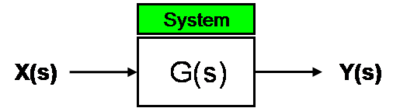
\includegraphics{images/400px-Transfer_Function_Block.png}
        \end{figure}
        Blocks like this fill the form of:

        \begin{align*} y(t) = g(t) * x(t) \Leftrightarrow Y(s) = G(s)X(s)\end{align*}

            % TODO: example on page 42.
        \begin{enumerate}
            \item Getting a Transfer Function:

            \begin{enumerate}
                \item Use theory to get equations to model the system
                \item Find equilibrium
                \item Linearize about equalibrium
                \item Take the Laplace Transform of the linearized equations with zero initial conditions
                \item Solve for $Y(s)$ in terms of $U(s)$, and eventually get $G(s)$
            \end{enumerate}

            \item Terminology:
                \begin{align*} G(s) = \frac{N(s)}{D(s)} \end{align*}

                \begin{enumerate}
                    \item rational $\iff n \text{ and } D$ are polynomials
                    \item proper $\iff deg(D) \ge deg(N)$
                    \item strictly proper $\iff deg(D) > deg(N)$
                    \item improper $\iff deg(N) > deg(D)$
                    \item poles are the roots of $D$
                    \item zeroes are the roots of $N$
                \end{enumerate}

            \item Obtaining the Transfer Function from the linear state model:

                \begin{align*}
                    \dot x = Ax + Bu &,& y = CX + Du
                \end{align*}
                Laplace transforms with zero initial coordinates are:

                \begin{align*}
                    sX(s) &= AX(s) + BU(s) \\
                    Y(s) &= CX(s) + DU(s) \\
                    (sI - A)X(s) &= BU(s) \\
                    X(s) &= (sI - A)^{-1} BU(s)
                \end{align*}
                By plugging this in to the function with $G$, we arrive at:
                \begin{align*}
                    Y(s) = CX(s) + DU(s) \\
                    \frac{Y(s)}{U(s)} = G(s) = \frac{CX(s)}{U(s)} + \frac{DU(s)}{U(s)} \\
                    G(s) = C(Is - A)^{-1} B + D \\
                    (\text{``Colin is a bad dog''})
                \end{align*}

            \item Interconnections/Substitutions in Block Diagrams: (See table)

                \begin{table}[h]
                    \centering
                    \begin{tabular}{ | l || l | l | l |}
                        \hline
                        Name & Equation & From & To \\ \hline

                        Series &
                            $Y = (P_1P_2)X$ &
                            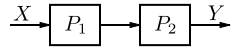
\includegraphics[width=40mm]{images/240px-Cascaded_Blocks.png} &
                            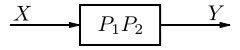
\includegraphics[width=40mm]{images/240px-Cascaded_Blocks_Equivalent.png} \\ \hline

                        Parallel &
                            $Y = P_1X \pm P_2X$ &
                            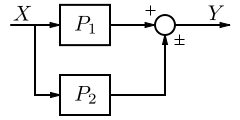
\includegraphics[width=40mm]{images/240px-Parallel_Blocks.png} &
                            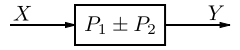
\includegraphics[width=40mm]{images/240px-Parallel_Blocks_Equivalent_1.png} \\ \hline

                        Moving Blocks &
                            $Z = PX \pm Y$ &
                            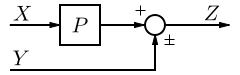
\includegraphics[width=40mm]{images/240px-Moving_Summing_Junction_in_front_of_Block_1.png} &
                            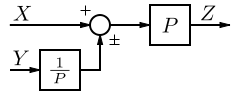
\includegraphics[width=40mm]{images/240px-Moving_Summing_Junction_in_front_of_Block_2.png} \\ \hline

                        Feedback &
                            $Y = P_1(X \mp P_2Y)$ &
                            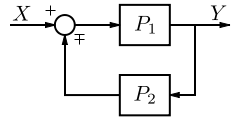
\includegraphics[width=40mm]{images/240px-Feedback_Loop.png} &
                            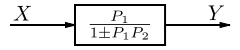
\includegraphics[width=40mm]{images/240px-Feedback_Loop_Equivalent_1.png} \\ \hline

                    \end{tabular}
                \end{table}

            \item Strategies for substituting diagrams with simpler diagrams

            \begin{enumerate}
                \item Introduce variables representing the output of summing junctions.
                \item Annotate inputs to the summers.
                \item Create equations per summer
                \item Solve all equations into 1 equation in terms of $\frac{Y(s)}{U(s)}$
            \end{enumerate}
        \end{enumerate}
    \item Linear System Theory

        \begin{enumerate}
            \item If $u(t)$ is a real-valued signal then it is bounded if $\exists b\ge 0$ such that $\forall t\ge 0 : |u(t)| \le b$
            % \item $u(t)$ for $t \ge 0$ is a real-valued signal $\iff$ $\lim_{t \to \infty} u(t) = c$, where $c$ is a constant.

            \item We can define BIBO stability such that for all bounded input, we produce bounded output.

            \item $G(s)$ is BIBO stable, and $G(s)$ is rational and strictly proper $\iff$ the impulse response $g(t) = \Lapm^{-1}\{G\}$ is absolutely integrable.

            \begin{align*} \int_0^{\infty} |g(t)| dt < \infty \Leftrightarrow \text{the system is BIBO stable}\end{align*}

            \item $G(s)$ is BIBO stable $\Leftrightarrow$ $G(s)$'s poles are complex numbers with $Re\{s\} < 0$.

            \item To prove that a given $G$ isn't BIBO stable, we need to find a bounded input $u(t)$ that produces an unbounded $y(t)$.

        \end{enumerate}
    \item Steady State Gain

        \begin{enumerate}
            \item A stable transfer function with $u(t) = u_0$ (constant, so $U(s) = \frac{u_0}{s}$) will have a steady state gain of $y_{ss}$.

                \begin{align*} \frac{y_{ss}}{u_0} = \frac{\lim_{t \to \infty} y(t)}{u_0} \end{align*}

                If G is stable, we can say:

                \begin{align*} y_{ss} = \lim_{t \to \infty} y(t)  = \lim_{s \to 0} sY(s) \end{align*}

            \item Steady state gain of stable systems equal $G(0)$, since $U(s) = \frac{u_0}{s}$, and the $s$ factors out, so:

                \begin{align*} \frac{y_{ss}}{u_0} = G(0) \end{align*}

        \end{enumerate}
    \item Steady state output for $u(t) = \cos(\omega t)$:

        For $u(t) = \cos(\omega t)$, and for stable $G(s)$, we can say that: $y_{ss} = A \cos(\omega t + \theta)$
            \begin{align*}
                u(t) &= e^{j\omega t} \\
                y_{ss}(t) &= g(t) * u(t) = \left( \int_{-\infty}^{\infty} g(\tau) e^{-j\omega \tau} d\tau \right) e^{j \omega t} \\
                \Rightarrow y_{ss}(t) &= G(j\omega)e^{j \omega t} \\
                &= |G(j\omega)|e^{j\phase{G(j\omega)}} e^{j \omega t} \\
                &= |G(j\omega)|e^{j  \left(\phase{G(j\omega)} + \omega t \right) } \\
                \Rightarrow y_{ss}(t) &= \frac{G(j\omega)e^{j  \omega t }}{2} + \frac{G(-j\omega)e^{-j  \omega t }}{2} \\
                &= Re\{ G(j\omega) e^{j  \omega t } \} \\
                y_{ss}(t) &= | G(j\omega) | \cos({\omega t + \phase{G(j \omega)}}) \\
            \end{align*}

        So, $A = |G(j \omega) |$, and $\theta = \phase{G(j \omega)}$

        $y_{ss}$ is a sin.

        We define the frequency response of $G$ as $G(j \omega)$
    \item Bode plots:

        \begin{enumerate}
            \item Bode plots give us an idea of how a system reacts to different kinds of input.

            \item Two kinds of plots are usually analyzed at the same time:

                \begin{itemize}
                    \item Magnitude plots compare the magnitude of the output (measured in dB) v.s. the frequency of the input:
                        \begin{align*} 20 \log{|G(j\omega)|} \text{ vs } \log(\omega) \end{align*}

                    \item Phase plots compare the angle (delay) of the output v.s. the frequency of the input:
                        \begin{align*} \phase{G(j\omega)} \text{ vs } \log(\omega) \end{align*}
                \end{itemize}

            \item We need this data to sketch Bode plots:

                \begin{itemize}
                    \item Pure Gain
                    \item Poles
                    \item First and Second Order Terms
                    \item Delays
                \end{itemize}

            \item Because $\log(|AB|) = \log(|A|) + \log(|B|)$ (and the same for angle), bode plots are additive.

                \begin{align*}
                    \log{ \left(\Pi_{q} (\text{simple term}_q) \right)} = \Sigma_q { \log{(\text{simple term}_q)}}
                \end{align*}

                We can then break these into a number of different cases which sum together: (refer to table)

                Remember: negative real poles/zeroes start out at $\pm 180 \textdegree$, not zero

                \begin{table}[h]
                    \centering
                    \begin{tabular}{ | p{5cm} || p{6cm} | p{6cm} |}
                        \hline
                        Term & Magnitude & Phase \\ \hline

                        Constant $ \left( K \right)$ &
                            $20 \log_{10}(|K|)$ &
                            $K < 0 ? 0\textdegree : \pm 180\textdegree$
                            \\ \hline

                        Pole at Origin $ \left( \frac{1}{s} \right)$ &
                            -20 dB/dec, $20\log(|G(j\omega)|) = 0$ when $\omega = 1$ &
                            -90\textdegree
                            \\ \hline

                        Zero at Origin $ \left( s \right)$ &
                            20 dB/dec, $20\log(|G(j\omega)|) = 0$ when $\omega = 1$ &
                            90\textdegree
                            \\ \hline

                        Real Pole $ \left( \frac{\omega_0}{s + \omega_0} \right)$ &
                            Asymptote at 0dB, goes to -20dB/dec at $\omega_0$ &
                            \parbox{5cm}{Asymptotes at 0\degree  and -90\degree \\ connect from $0.1 \omega_0$ to $10 \omega_0$}
                            \\ \hline

                        Real Zero $ \left( \frac{s + \omega_0}{\omega_0} \right)$ &
                            Asymptote at 0dB, goes to  +20dB/dec at $\omega_0$ &
                            \parbox{5cm}{Asymptotes at 0\degree  and +90\degree \\ connect from $0.1 \omega_0$ to $10 \omega_0$}
                            \\ \hline

                        Underdamped Poles $ \left( \frac{\omega_0^2}{s^2 + 2 s \zeta \omega_0 + \omega_0^2} \right)$, $0 < \zeta < 1$ &
                            \parbox{6cm}{
                                Asymptote at 0dB, another (non-const) asymptote at -40dB/decade. \\
                                Generally, they intersect at $\omega_0$, but if $\zeta > 0.5$, there is a peak at: $|G(j\omega_0)| = -20 \log_{10}(2\zeta)$
                            } &
                            \parbox{5cm}{
                                Low frequency asymptote at 0\degree  and -180\degree \\ connect from $ \frac{\omega_0}{5^\zeta}$ to ${\omega_0}{5^\zeta}$}
                            \\ \hline

                        Underdamped Zeros $ \left( \frac{1}{\omega_0^2}  {(s^2 + 2 s \zeta \omega_0 + \omega_0^2)} \right)$, $0 < \zeta < 1$ &
                            \parbox{6cm}{
                                Asymptote at 0dB, another (non-const) asymptote at 40dB/decade. \\
                                Generally, they intersect at $\omega_0$, but if $\zeta > 0.5$, there is a peak at: $|G(j\omega_0)| = 20 \log_{10}(2\zeta)$
                            } &
                            \parbox{5cm}{
                                Low frequency asymptote at 0\degree  and 180\degree \\ connect from $ \frac{\omega_0}{5^\zeta}$ to ${\omega_0}{5^\zeta}$}
                            \\ \hline

                        Delay $ \left( e^{-j\omega_0t} = \cos(\omega_0 t) - j\sin(\omega_0 t) \right)$ &
                            ``Flatlined'' at 0dB &
                            Grows linearly with time, but log plot makes it look curved.
                            \\ \hline

                    \end{tabular}
                \end{table}

                The general strategy for drawing bode plots is:

                \begin{enumerate}
                    \item Rewrite $G(s)$ in the proper form (multiplication of simpler terms)
                    \item Separate the transfer function into constituent parts.
                    \item Draw the bode diagram of each part.
                    \item The overall bode diagram is the sum of all parts.
                    \item Rejoice! You are done the question.
                \end{enumerate}
            \item Time response of $1^{st}$ order ODEs:

                Recall, first-order systems are the form of:
                \begin{align*}
                    \tau \dy + y = Ku &\Rightarrow^{\Lapm} G(s) = \frac{K}{1+s\tau} \\
                \end{align*}

                \begin{enumerate}
                    \item We measure the output settling to the asymptote (usually $y_{ss}$) in response to a step function.

                    \item We define bandwidth as $\tau^{-1}$.

                    \item We measure the time response as a comparison between $y_{ss}$ and an initial state of $0$.

                    \item As $\tau$ increases, the time response becomes faster.

                    \item We define the settling time as when the output settles to $2 \%$ of the asymptote.

                    \item There is no peaking (or ``overshoot'') in first-order systems.

                    \item As $\tau$ approaches 0, the pole $s = -\tau^{-1}$ moves to the left.

                    \item Settling time = $4\tau$

                    \item TL;DR:
                        \begin{enumerate}
                            \item Stable at $\tau > 0$.
                            \item Pole at $s = \frac{-1}{\tau}$.
                            \item Bandwidth $\approx \frac{1}{\tau}$.
                            \item No overshoot or oscillation in step response.
                            \item Settling time = $4\tau$
                        \end{enumerate}
                \end{enumerate}
            \item Time response of $2^{nd}$ order ODEs: ($\forall \zeta$)

                Recall, second-order systems can be written in the form:
                \begin{align*}
                    G(s) = \frac{K \omega_n^2}{s^2 + 2s\omega_n \zeta + \omega_n^2} \\
                \end{align*}
                \begin{enumerate}
                    \item Poles are at $s = -\zeta \omega_n \pm \sqrt{\zeta^2 - 1}$
                    \item Pole behaviour:
                    \begin{enumerate}
                        \item $0 < \zeta < 1$ : complex conjugate : under-damped
                        \item $\zeta = 1$ : 2 real repeated poles : critically damped
                        \item $\zeta > 1$ : 2 real distinct poles : over-damped
                    \end{enumerate}
                    \item Angle: $\theta = \cos^{-1}(\zeta)$.
                    \item $\zeta$ is the damping ratio.
                    \item $\omega_n$ is the undamped natural frequency, and the bandwidth.
                    \item As $\omega_n$ incresases (larger bandwidth), the time response is faster.
                \end{enumerate}

                \begin{enumerate}
                    \item $ 0 < \zeta < 1$ (underdamped systems):
                        \begin{itemize}
                            \item Impulse response:
                                \begin{align*}
                                    g(t) &= \Lapm^{-1}\{G(s)\} \\
                                    &= \frac{k\omega_n}{\sqrt{1-\zeta^2}} e^{-\zeta \omega_n \tau} \sin(\omega_n \tau \sqrt{1-\zeta^2} )
                                \end{align*}
                            \item Step Response: ($u(t) = $ heaviside)
                                \begin{align*}
                                    y(t) &= \Lapm^{-1} \left\{ G(s) \frac{1}{s} \right\}
                                    \\&= \text{something very complicated}
                                \end{align*}
                            \item Poles are complex conjugates.
                            \item As $\zeta$ approaches $1$, the time response oscillates less. Vice versa holds.
                            \item Zeros: none
                            \item Magnitude of poles: $\cdots = \omega_n$.
                            \item DC gain: $G(0) = k$
                            \item Frequency response: Bandwidth $\approx \omega_n$
                        \end{itemize}

                    \item $ \zeta > 1$ (overdamped systems):

                        \begin{align*} G(s) = \frac{kab}{(s+a)(s+b)} \end{align*}
                        \begin{itemize}
                            \item Impulse response:
                                \begin{align*} g(t) = \Lapm^{-1}\{G(s)\} = \frac{kab}{b-a} (e^{-a \tau} - e^{-b \tau} ) \end{align*}
                            \item Step Response: ($u(t) = $ heaviside)
                                \begin{align*} y(t) = \Lapm^{-1} \left\{ G(s) \frac{1}{s} \right\} = k \left(1 + \frac{1}{b-a} (ae^{-bt} - be^{-at}) \right) \end{align*}
                            \item Zeros: none
                            \item DC gain: $G(0) = k$
                            \item 2 real distinct poles
                            \item As $\zeta$ approaches $1$, the time response oscillates less. Vice versa holds.
                            \item no overshoot, no oscilations
                            \item bandwidth = min$(a, b)$
                        \end{itemize}

                    \item $ \zeta = 1$ (critically damped systems):

                        \begin{align*} G(s) = \frac{ka^2}{(s+a)^2} \end{align*}
                        \begin{itemize}
                            \item Poles: $s = -\zeta \omega_n = -\omega_n$
                            \item Zeros: none
                            \item slower than overdamped/underdamped systems to converge
                            \item DC gain: $G(0) = k$
                            \item 2 real \& identical poles
                            \item As the bandwidth ($\omega_n$) increases, the time response is faster.
                            \item no overshoot, no oscilations
                            \item bandwidth = $a$
                        \end{itemize}
                \end{enumerate}
            \item Characteristics of a step response

                \begin{enumerate}
                    \item Common metrics apply to any system when we evaluate it.
                    \item Higher order systems can be approximated as 2nd order systems.
                    \begin{figure}[h]
                        \centering
                        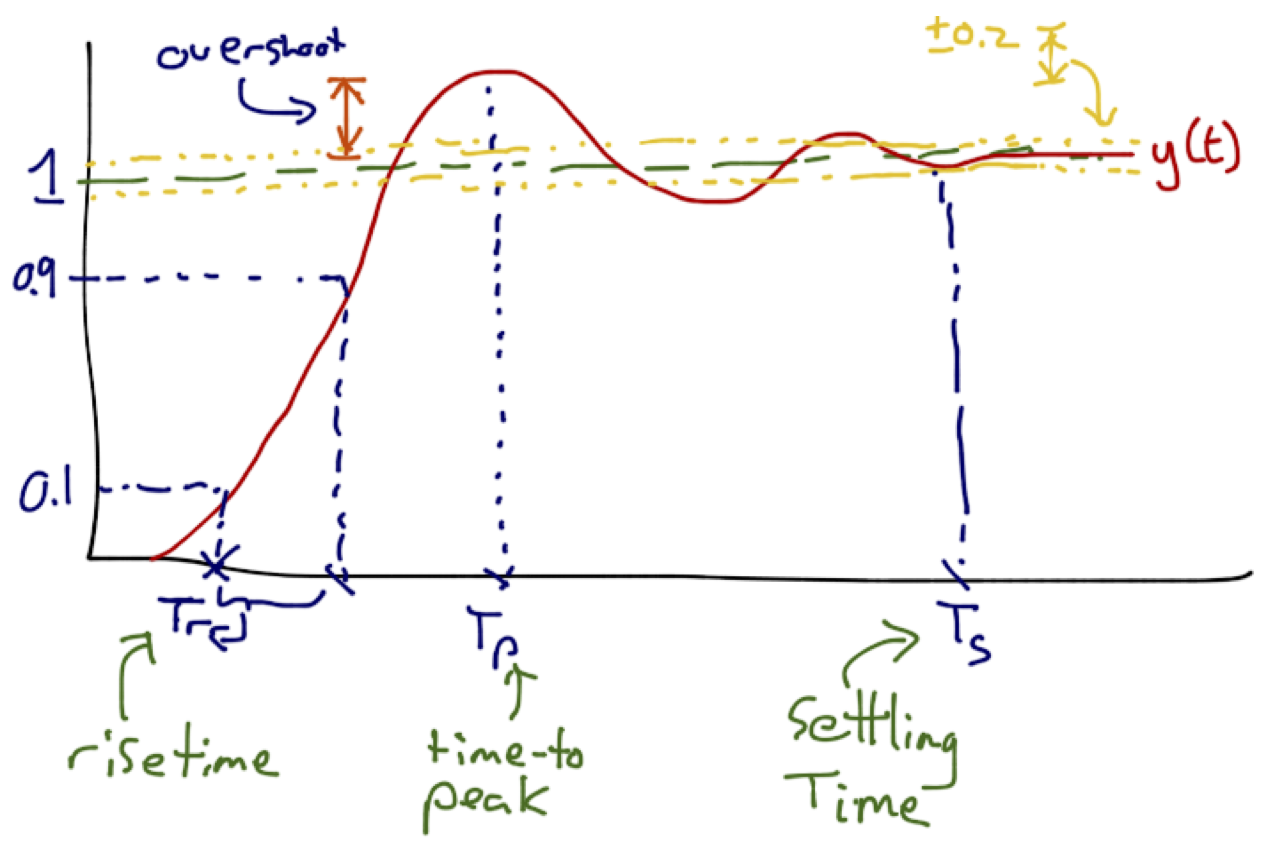
\includegraphics[width=0.75\textwidth,height=0.25\textheight,keepaspectratio]{images/timing.png}
                    \end{figure}
                    \item Overshoot ($\% OS$):

                        \begin{itemize}
                            \item Only underdamped systems have overshoot.
                            \item We find the first $\dy = 0$, and plug that into $y(t)$

                            \item Generally, we have:

                                \[
                                     \% OS = \frac{M_p - K}{K} = \exp \left( \frac{-\zeta \pi}{\sqrt{1-\zeta^2}} \right)
                                \]
                        \end{itemize}

                    \item Settling Time ($T_s$)

                        \begin{itemize}
                            \item Amount of time it takes for a response to lie within 2\% of $y_{ss}$
                            \item Crude estimate: $t \ge \frac{4}{\zeta \omega_n}$

                            \begin{align*}
                                T_s = \frac{4}{\zeta \omega_n}
                            \end{align*}
                        \end{itemize}

                    \item Time To Peak ($T_p$)

                        \begin{itemize}
                            \item Time it takes to reach the max value.
                            \item Only depends on imaginary part of the poles:

                            \begin{align*}
                                T_p = \frac{\pi}{\omega_n \sqrt{1 - \zeta^2}}
                            \end{align*}
                        \end{itemize}

                    \item Rise Time ($T_r$)

                        \begin{itemize}
                            \item Time it takes to go from 10\% to 90\% of $y_{ss}$ from $0$, valid for $0.3 \le \zeta \le 0.8$

                            \begin{align*}
                                T_r \approx \frac{2.16\zeta + 0.6}{\omega_n}
                            \end{align*}
                        \end{itemize}
                \end{enumerate}
        \end{enumerate}

    Space intentionally left blank. [didn't take notes the day before the midterm]
    \item Adding Zeros:
        \begin{itemize}
            \item Adding a minimum phase Zero:
                \begin{align*}
                    G_a(s) &= G(s) (1 + \tau s), \tau > 0 \\
                    &= \frac{k \omega_n^2}{s^2 + 2 \zeta \omega_n s + \omega_n^2}
                \end{align*}
                TODO: insert graph of this from class.
                We use $\tau > 0$ so that $\frac{-1}{\tau}<0$ (i.e. the introduced zero is in the left-half plane)
                \begin{itemize}
                    \item Step response:
                        \begin{align*}
                            y(t) &= \Lapm^{-1} \left\{ \frac{G_a(s)}{s} \right\} \\
                            &= \Lapm^{-1} \left\{ \frac{G(s)}{s} + \frac{\tau s G(s)}{s} \right\} \\
                            &= (\text{step response of $G(s)$} ) + \tau(\text{impulse response of $G(s)$})
                        \end{align*}
                        As $\tau \rightarrow 0$, $G_a(s)$ approaches the step response of $G(s)$. \\
                        Likewise, as $\tau \rightarrow \infty$, $G_a(s)$ approaches the impulse response of $G(s)$.

                        This makes the phase plot more positive, and the magnitude plot ``rolls off'' slower. The bandwidth increases.

                        In all, the system becomes faster, but with the penalty of overshoot.

                        Knowing these attributes when designing PID controllers helps us understand that we want more 0's.
                \end{itemize}

        \end{itemize}
    \item  Feedback Control.

            \begin{itemize}
                \item ... Notes in PDF
                \item The most fundamental spec is stability.

                Good performance usually requires high gain but can also lead to instability.

                \item Two approaches to design/analysis:

                \begin{enumerate}
                    \item Classical

                        This course, freq domain, specs are based on closed-loop bandwidth, stability, margins. Design done with Bode plots.

                    \item Modern:

                        State Space (ECE 488)
                        In time domain, specs are in terms of pole locations.
                \end{enumerate}
                    The approaches are complementary.

                \begin{enumerate}

                    \item Classical: good SISO (single input, single output) systems, and open loop stable plants.

                    \item Modern: MIMO systems, and unstable plants

                \end{enumerate}

                \item Example:

                    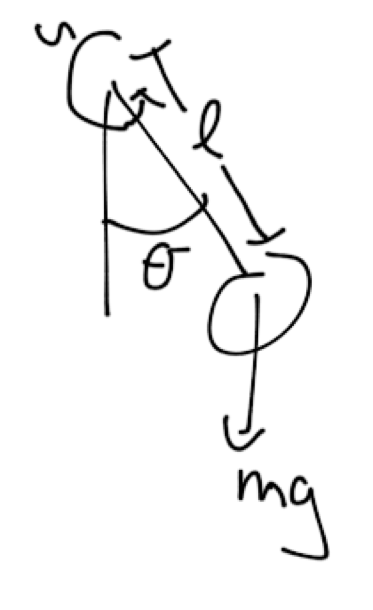
\includegraphics[width=90px,keepaspectratio]{images/5-1.png}

                    Since we want to control position, I take the output $y = \Theta$. $y = x_1 = \Theta$

                    The model is (Problem Set 2):
                    ($J$ is the inertia of the system?)
                    \begin{align*}
                        \dx_1 = x_2 \\
                        \dx_2 = \frac{-mgl \sin{x_1}}{J} + \frac{u}{J} \\
                        y = x_1
                    \end{align*}

                    The upright position is $x_1 =\pi$. The equilibrium corresponding to this is found by solving:

                    \begin{align*}
                        0 = f(x_0, u_0) \\
                        y = h(x_0, u_0)
                    \end{align*}

                    For $x_0 = (x_{01}, x_{02})$, we get (problem set 2):

                    \begin{align*}
                        x_0 = [\pi, 0]  \\
                        u_0 = 0
                    \end{align*}

                    Let $dx = x - x_0$ \text{, } $dy = y - y_0$ \text{, } $du = u - u_0$.

                    The linearized model is (Problem set 3):

                    \begin{align*}
                        dx(dot) &= \begin{bmatrix} 0 & 1 \\ \frac{mgl}{J} & 0  \end{bmatrix} dx + \begin{bmatrix} 1 \\ \frac{1}{J} \end{bmatrix} du \\
                        dy &= \begin{bmatrix} 1 \\ 0 \end{bmatrix} dx
                    \end{align*}

                    Let $Y(s) = \Lapm\{dy\}$, $U(s) = \Lapm\{du\}$.

                    \begin{align*}
                        \frac{Y(s)}{U(s)} = \frac{1/J}{s^2 - \frac{mgl}{J}} = P(s) \\
                        \text{(problem set 3)}
                    \end{align*}

                    The poles are $s = \pm \sqrt{\frac{mgl}{J}}$

                    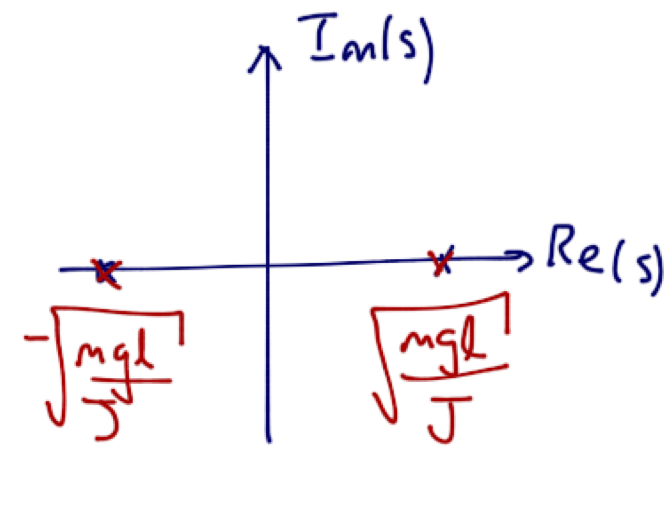
\includegraphics[width=90px,keepaspectratio]{images/5-2-a.png}

                    This implies that the plant is unstable.

                    The block diagram so far.

                    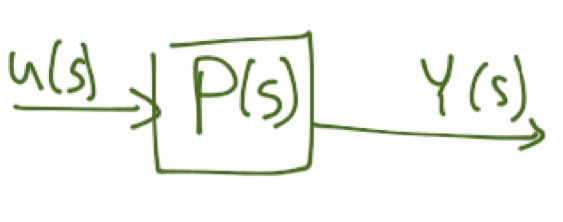
\includegraphics[width=90px,keepaspectratio]{images/5-2-b.png}

                    Let's try and stabilize the system by feeding back the position (using an encoder) and comparing it to reference $r$, and using the error $r-y$ to drive our controller

                    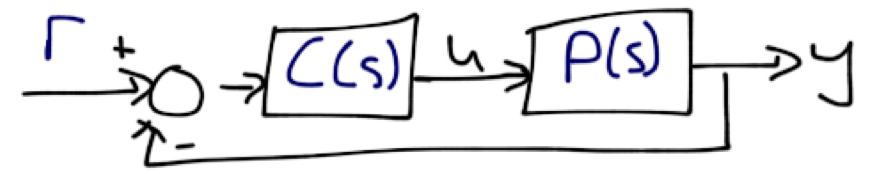
\includegraphics[width=90px,keepaspectratio]{images/5-2-c.png}

                    One controller that works is (for simplicity, assume $J = 1$, $mgl = 1$)

                    \begin{align*}
                        C(s) = 100  \frac{s+10}{s+20}
                    \end{align*}
                    Called a lead controller

                    With this $C(s)$, the TF from $R$ to $Y$ is:

                    \begin{align*}
                        \frac{Y(s)}{R(s)} =
                        \frac{100s + 1000}{s^3 + 20s^20s + 99s + 980}
                    \end{align*}

                    The poles of this transfer function are $\{ -17.5, -1+j7.3, -1 - j7.3\}$

                    \begin{center}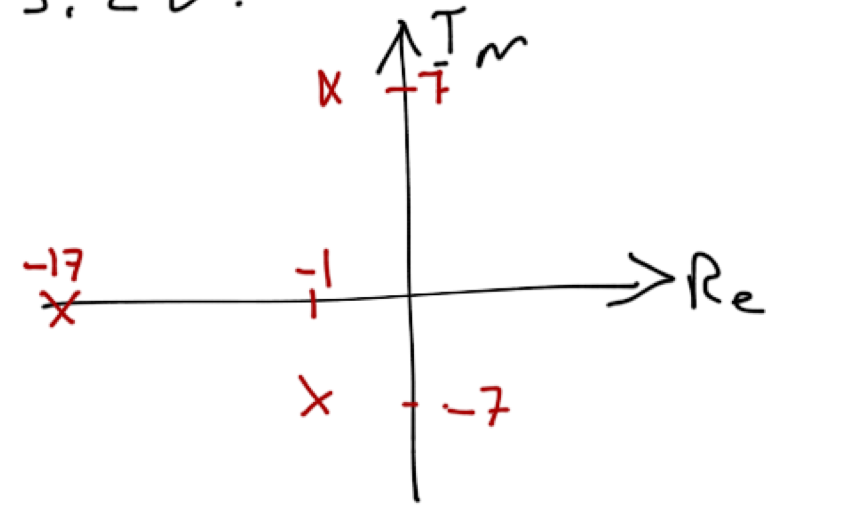
\includegraphics[width=0.5\textwidth,keepaspectratio]{images/5-2-d.png}\end{center}

                    So by CH3, the system is BIBO stable. (all poles are in LHP).

                    Based on CH4, we expect a very oscillatory step response. The pole at $s = -17$ will have very little effect.

                    Let's apply $r(t) = 1(t) - 1(t-5)$:

                    \begin{center}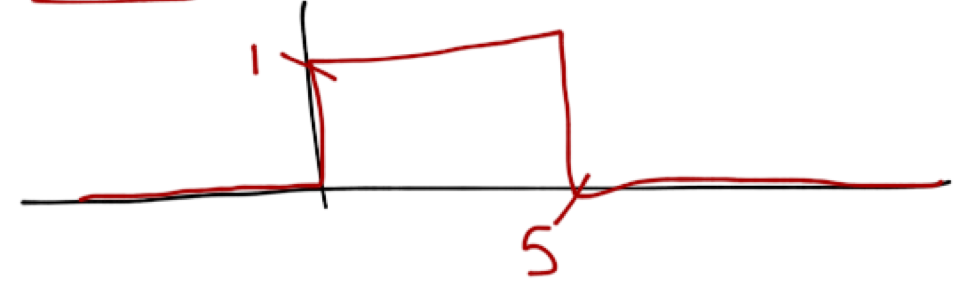
\includegraphics[width=0.5\textwidth,keepaspectratio]{images/5-2-e.png}\end{center}

                    $\rightarrow$ move pendulum to $dy = 1$ for $t \in [0, 5]$ (56 \textdegree), then back to upright position $dy = 0$ for $t > 5$.

                    \begin{center}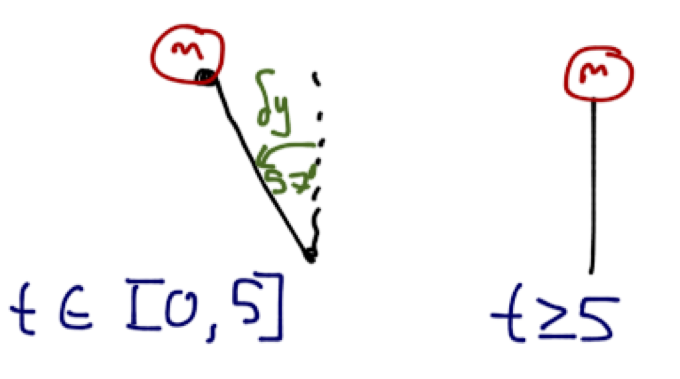
\includegraphics[width=0.5\textwidth,keepaspectratio]{images/5-2-f.png}\end{center}

                    The step response (he used Matlab):

                    \begin{center}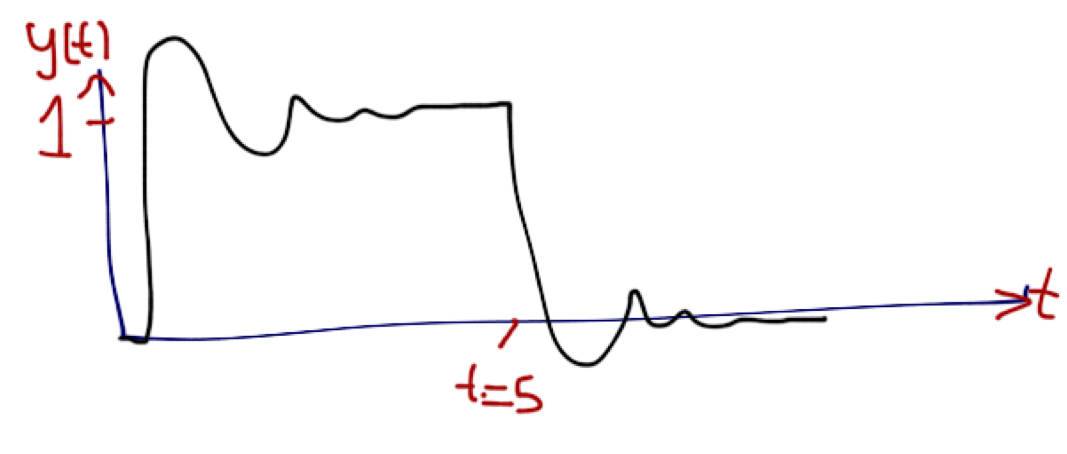
\includegraphics[width=0.5\textwidth,keepaspectratio]{images/5-2-g.png}\end{center}

            \end{itemize}

        \item Closing the loop (a detailed example)

            \begin{center}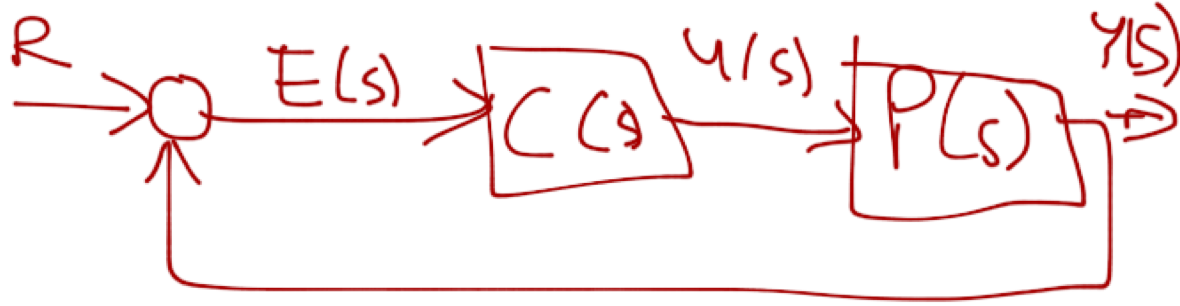
\includegraphics[width=0.5\textwidth,keepaspectratio]{images/5-1-false.png}\end{center}

            If $E(s) = R(s) - Y(s)$, then $\frac{U(s)}{E(s)} = C(s) = 100 \frac{s + 10}{s+20}$

            \begin{align*}
                \dot u + 20u = 100 \dot e + 1000e \\
            \end{align*}

            This means that this ODE needs to be implemented in software. Typically done by discretizing and approximating the ODE.

            The most common way to implement the ODE is to use the ``trapezoidal approximation''

            \begin{center}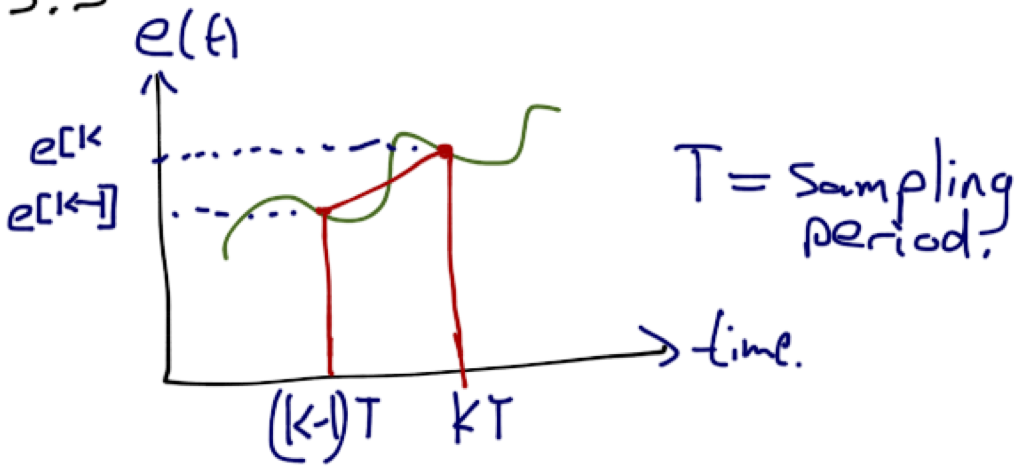
\includegraphics[width=0.5\textwidth,keepaspectratio]{images/5-3.png}\end{center}

            \begin{align*}
                \int^{k \tau }_{(k-1) \tau )} e( \tau )d \tau &\approx \frac{T}{2} \left( e[k] + e[k-1] \right)
            \end{align*}

            This generates a ``rule'':

            \begin{align*}
                s = \frac{2}{T} \frac{z - 1}{z + 1}
            \end{align*}

            Where $s$ is the laplace variable, and $z$ is the $z$-transform variable.

            In this case we get:

            \begin{align*}
                \frac{U[z]}{E[z]} &= C[z] \\
                 &= C(s)\Big|_{s = \frac{2}{T} \frac{z - 1}{z + 1}} \\
                 &= \frac{100 ((1+5T) + (5T - 1)z^{-1})}{((1+10T) + (10T -1) z^{-1})}
            \end{align*}

            Taking the inverse z-transform, we get:

            \begin{align*}
                (1+10T) u[k] + (10T-1)u[k-1] = 100 (1+5T)e[k] + 100(5T - 1) e[k-1]
            \end{align*}
            If $T > 0$ is small, the controller works well.

        \item Feedback stability:

            \begin{center}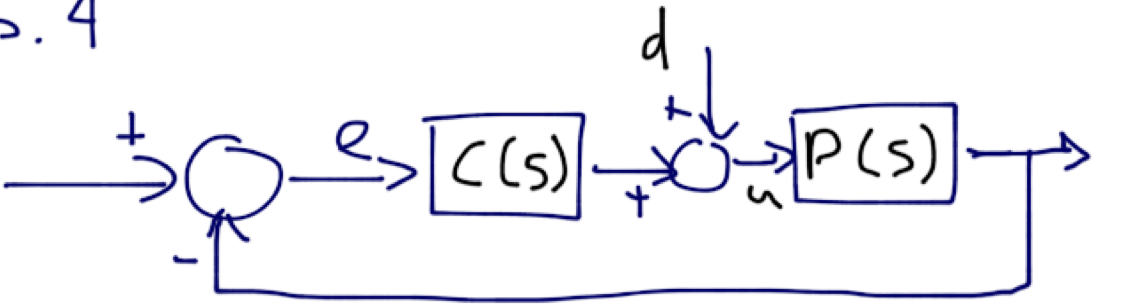
\includegraphics[width=0.5\textwidth,keepaspectratio]{images/5-4.png}\end{center}

            Where $P(s)$ is the plant \\
            Where $C(s)$ is the controller \\
            $r(t)$ is the reference \\
            $e(t)$ is the tracking error \\
            $d(t)$ is the disturbance \\
            $u(t)$ is the control input \\
            $y(t)$ is the output

            6 Transfer functions associated with this system $(r, d) \to (e, u, y)$

            \begin{enumerate}
                \item $\frac{R}{E} = \frac{1}{1+PC}$
                \item $\frac{D}{E} = \frac{-P}{1+PC}$
                \item $\frac{R}{U} = \frac{C}{1+PC}$
                \item $\frac{D}{U} = \frac{1}{1+PC}$
                \item $\frac{R}{Y} = \frac{PC}{1+PC}$
                \item $\frac{D}{Y} = \frac{P}{1+PC}$
            \end{enumerate}

            We make the standing assumption that $C(s)$, $P(s)$ are rational, and $C(s)$ is proper, and $P(s)$ is strictrly proper, and the 2x2 matrix below has a non-zero determinant.

            Equations at the output summers:
            \begin{align*}
                E &= R - PU \\
                U &= D + CE \\
                \begin{bmatrix} 1 & P \\ -C & 1  \end{bmatrix} \begin{bmatrix} E \\ U  \end{bmatrix} &= \begin{bmatrix} R \\ D  \end{bmatrix}
            \end{align*}

            In light of our assumptions, we have the following:
            \begin{align*}
                \begin{bmatrix} E \\ U  \end{bmatrix} &= {\begin{bmatrix} 1 & P \\ -C & 1  \end{bmatrix}}^{-1} \begin{bmatrix} R \\ D  \end{bmatrix} \\
                &= {\begin{bmatrix} \frac{1}{1+PC} & \frac{-P}{1+PC} \\ \frac{C}{1+PC} & \frac{1}{1+PC}  \end{bmatrix}} \begin{bmatrix} R \\ D  \end{bmatrix}
            \end{align*}

            The output is:
            \begin{align*}
                Y &= PU \\
                &= \frac{PC}{1+PC}R + \frac{D}{1 + PC}D
            \end{align*}

            We can define the system as {\bf feedback stable} if for every bounded $r$ and $d$, we have bounded $(u, e, y)$.

            Since whenever $r$ and $e$ are bounded, $y = r - e$ is also bounded, it suffices to look at the 4 Transfor functions from $(r, d) \to (u, e)$.

            {\bf Example}:
            \begin{align*}
                P(s) &= \frac{1}{s^2 -1} \\
                C(s) &= \frac{s-1}{s+1}
            \end{align*}

            The 4 transfer functions are:
            \begin{align*}
                \begin{bmatrix}
                    \frac{(s+1)^2}{s^2 + 2s + 2} &
                    \frac{s+1}{(s+1)(s^2 + 2s + 2)} \\
                    \frac{(s+1)(s-1)}{s^2 + 2s + 2} &
                    \frac{(s+1)^2}{s^2 + 2s + 2}
                \end{bmatrix}
            \end{align*}

            Three of the transfer functions are BIBO stable, the one from $D$ to $E$ is {\uline not}. This is in spite of the fact that a bounded $r$ produces a bounded $y$. Notice that $C(s)$ cancels an unstable pole in $P(s)$.

            We'll see that this doesn't work.

        \item Testing for feedback stability:

            Write $P(s) = \frac{N_p}{D_p}$, and $C(s) = \frac{N_c}{D_c}$

            Assume:

            \begin{itemize}
                \item $(N_p, D_p)$ are \uline{coprime} (i.e. no common factors)
                \item $(N_c, D_c)$ are \uline{coprime} too.
            \end{itemize}

            The \uline{characteristic polynomial} (he writes ch.p) of the feedback system is:

            \begin{align*} \Pi(s) = N_p N_c + D_p D_c\end{align*}
            He calls this ``unity feedback''.

            The characteristic polynomial is the denominator of the 4 Transfer functions $(r,d) \to (e, u)$

            \begin{align*}
                \begin{bmatrix} \frac{1}{1+PC} & \frac{-P}{1+PC} \\ \frac{C}{1+PC} & \frac{1}{1+PC}  \end{bmatrix} &=
                \frac{1}{\Pi(s)} \begin{bmatrix}
                    D_p D_c & -N_p D_c \\
                    N_c D_p & D_p D_c
                \end{bmatrix}
            \end{align*}

            \begin{itemize}
                \item \example $P(s) = \frac{1}{s^2-1}$, $C(s) = \frac{s-1}{s+1}$

                    \begin{align*}
                        \Pi(s) &= (s-1) + (s^2 -1) (s+1) \\
                        &= (s-1)(s^2 + 2s + 2)
                    \end{align*}

                    $s-1$ is unstable, thus this is unstable.

                \item \theorem The feedback system is stable if and only if the \chpm has no roots in $\{ s \in \mathbbold{C}. \text{Re}(s) \ge 0 \}$
                \item \proof of theorem:
                    \begin{itemize}
                        \item ($\leftarrow$)

                            If $\Pi(s) = N_p N_c + D_p D_c$ has no roots with $\text{Re}(s) \ge 0$, then the 4 transfer functions $ (r,d) \to (e,u)$ are BIBO stable and hence the feedback system is stable.

                        \item ($\rightarrow$)

                            Assume the feedback system is stable, i.e. the 4 TFs $(r, d) \to (e, u)$ are BIBO stable.
                            To conclude that $\Pi(s)$ has no roots in $\text{Re}(s) \ge 0$, we must conclude show that $\Pi(s)$ \uline{has no common roots} with the numerators $D_p D_c$, $N_c D_p$, $N_p D_c$

                            He leaves this proof to us (as an excercise to the reader).
                    \end{itemize}
                \item \defi{Pole-Zero Cancellation}:

                    The plan $P(s)$, and controller $C(s)$ have a \uline{pole-zero cancellation} at $\lambda \in \mathbbold{C}$.
                    If $N_p(\lambda) = D_c(\lambda) = 0$, then the controller pole cancels the plant zero.
                    If $N_c(\lambda) = D_p(\lambda) = 0$, then the controller zero cancels the plant pole.
                \item \defi{Unstable pole-zero cancellation}

                    It's called an \uline{unstable pole-zero cancellation} if $Re(\lambda) \ge 0$.

                \item \corollary If there is an unstable pole-zero cancellation, then the feedback system is unstable.

                \item \proof
                    Suppoe there is an unstable cancellation at $\lambda \in \mathbbold{C}$, with $\text{Re}(s) \ge 0$.
                    Then:

                    \begin{align*}
                        \Pi(\lambda) &= N_c(\lambda) N_p(\lambda) + D_c(\lambda) D_p(\lambda) \\
                        &= 0 + 0 \\
                        &= 0
                    \end{align*}

                    Hence $\Pi$ has a root with $\text{Re}(s) \ge 0$, so by previous theorem, the feedback system is unstable.

                \item \theorem The feedback system is stable iff:
                    \begin{itemize}
                        \item The TF $1 + PC$ has no zeros with $\text{Re}(s) \ge 0$
                        \item There are no unstable pole-zero cancellations
                    \end{itemize}

                \item \example $P(s) = \frac{1}{s^2 -1}$, $C(s) = \frac{s-1}{s+1}$

                    There are unstable pole-zero cancellations, so this must not be stable.

                \item \rmk Sometimes, we model the sensor as follows:

                    \begin{center}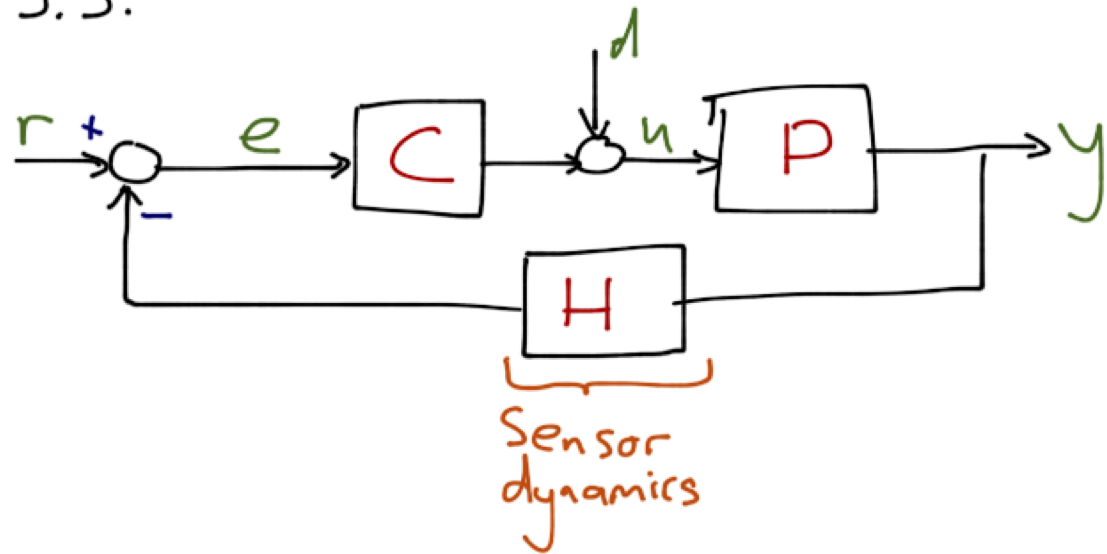
\includegraphics[width=0.5\textwidth,keepaspectratio]{images/5-5.png}\end{center}

                    We write:

                    \begin{align*}
                        P &= \frac{N_p}{D_p} \\
                        C &= \frac{N_c}{D_c} \\
                        H &= \frac{N_h}{D_h}
                    \end{align*}
            \end{itemize}

        \item 5.12: Comparison of open-loop and closed-loop poles/zeros:

            \begin{center}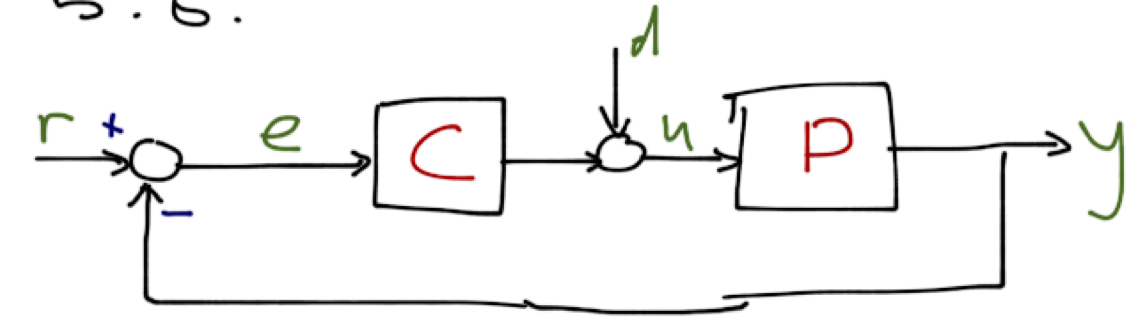
\includegraphics[width=0.5\textwidth,keepaspectratio]{images/5-6.png}\end{center}

                We write:

                \begin{align*}
                    P &= \frac{N_p}{D_p} \\
                    C &= \frac{N_c}{D_c}
                \end{align*}

            The open-loop TF is $PC = \frac{N_p N_c}{D_p D_c}$.

            The closed-loop TF is $\frac{PC}{1+PC} = \frac{N_p N_c}{D_p D_c + N_p N_c}$.

            Observations:

            \begin{itemize}
                \item The zeroes of closed-loop system equals of the zeros of an open-loop system (except the ones that were cancelled).

                \item If P has a non-minimum phase zero, so does the closed-loop system.

                \item Usually, we design our poles to be in a good region.
            \end{itemize}

        \item 5.2 The Routh-Hurwitz Stability Criterion
            \begin{enumerate}
                \item In practice, we often check feedback stability by numerically computing roots of $\Pi(s)$
                \item If some of the coefficients of $\Pi(s)$ are not fixed, e.g. controller gains we can't compute numerical solutions
                \item The right hand test provides a way to check if the roots of a polynomial are in $\mathbbold{C}^-$. This test is useful for design.


                \item Example of a $1^{st}$ order:

                        \begin{align*}
                            \Pi(s) &= a_1 s + a_0 \\
                            a_1 &\ne 0 \\
                        \end{align*}
                        The root is $s = \frac{-a_0}{a_1}$.

                        So $\Pi(s)$ is stable $\Leftrightarrow$ sign($a_1$) = sign($a_0$).

                \item Example of a $2^{nd}$ order:

                        \begin{align*}
                            \Pi(s) &= a_2 s^2 + a_1 s + a_0 \\
                            a_2 &\ne 0 \\
                        \end{align*}
                        The roots are $s = \frac{-a_1 \pm \sqrt{a_1^2 - 4 a_2 a_0}}{2 a_2}$.
                        We know that sign($a_1$) = sign($a_0$).

                        It's no longer obvious what the conditions are on $a_2$, $a_1$, $a_0$ should be.

                \item Algorithm:

                    Consider the general characteristic polynomial:
                    \begin{align*}
                        \Pi(s) &= \sum_{i=0}^{n} a_i s^i \\
                        &= a_0 + a_2 s^2 + a_3 s^3 + \ldots + a_n s^n \\
                        a_i &\in \mathbbold{R}
                    \end{align*}

                    A necessary condition for $\Pi(s)$ to have all it's roots in $\mathbbold{C}^-$ is that all the $a_i$'s have the same sign.

                    To tee this, factor $\Pi(s)$ as follows:

                    \begin{align*}
                        \Pi(s) &= a_n (s-\lambda_1) \ldots (s-\lambda_r)(s-\mu_1)(s-\bar{\mu_1}) \ldots (s-\mu_s)(s-\bar{\mu_s})
                    \end{align*}

                    Where $\{ \lambda_1, \ldots, \lambda_r \}$ are the real roots, and
                    $\{ \mu_1, \bar{\mu_1}, \ldots, \mu_r, \bar{\mu_r} \}$ are the complex conjugate roots.

                    $n = r + 2s$.

                    If $\lambda_i < 0$, then $- \lambda_i > 0$

                    If Re($\mu_i$) = Re($\bar{\mu_i}$), then we know that $(s - \mu_i)(s - \bar{\mu_i}) = s^2 - (\mu_i + \bar{\mu_i}) s + \mu_i \bar{\mu_i}$.

                    We know that $(\mu_i + \bar{\mu_i}) > 0$, and $ \mu_i \bar{\mu_i}$ > 0.

                    If we re-expand the polynomial, we see that all coefficients have sign($a_n$).

                \item General way to set up a Routh-Hurwitz table:

                    Zig-zag the first two rows that coefficients are placed in.
                    \begin{align*}
                        \Pi(s) = \sum_i^n a_i s^i
                    \end{align*}
                    \begin{table}[h]
                        \centering
                        \begin{tabular}{ | l || l | l | l | l | l | }
                            \hline
                            \hline
                            $s^n$ & $a_n$ & $a_{n-2}$ & $a_{n-4}$ & \ldots & $a_0$ \\ \hline
                            $s^{n-1}$ & $a_{n-1}$ & $a_{n-3}$ & $a_{n-5}$ & \ldots & $0$\\ \hline
                        \end{tabular}
                    \end{table}

                    Calculate elements using the negative determinant of the far-left column directly above and the column one to the right and above, divided by the one directly above at the far left:

                    \begin{table}[h]
                        \centering
                        \begin{tabular}{ | l || l | l | l | l | l | }
                            \hline
                            \hline
                            $s^i$ & $a_{(i, 0)}$ & $a_{(i, 1)}$  & $a_{(i, 2)}$ & \ldots \\ \hline
                            $s^{i-1}$ & $a_{(i-1, 0)}$ & $a_{(i-1, 1)}$  & $a_{(i-1, 2)}$ & \ldots \\ \hline
                            $s^{i-2}$ & $a_{(i-2, 0)}$ & $a_{i-2, 1}$  & $a_{i-2, 2}$ & \ldots \\ \hline
                        \end{tabular}
                    \end{table}

                    We have:
                    \begin{align*}
                        a_{(j, k)} &= \frac{-\begin{vmatrix} a_{(j-2, 0)} & a_{(j-2, k+1)} \\ a_{(j-1, 0)} & a_{(j-1, k+1)}  \end{vmatrix}}{a_{(j-1, 0)}}
                    \end{align*}

                    For example:
                    \begin{align*}
                        \Pi(s) &= a_3 s^3 + a_2 s^2 + a_1 s + a_0
                    \end{align*}
                    \begin{table}[h]
                        \centering
                        \begin{tabular}{ | l || l | l | l | l | l | }
                            \hline
                            \hline
                            $s^3$ & $a_3$ & $a_1$ & $0$ \\ \hline
                            $s^2$ & $a_2$ & $a_0$ & $0$ \\ \hline
                            $s^1$ & $\frac{a_2 a_1 - a_3 a_0}{a_2}$ & $0$ & $0$ \\ \hline
                            $s^0$ & $a_0$ & $0$ & $0$ \\ \hline
                        \end{tabular}
                    \end{table}

                    We need all roots to be in the LHP to be stable, so we want to pick the values as follow:

                    $a_3 > 0$, $a_2 > 0$, $\frac{a_2 a_1 - a_3 a_0}{a_2} > 0$, $a_0 > 0$

                \item C, P example:

                    \begin{align*}
                        P &= \frac{2}{s^2 + s + 1} \\
                        C &= K_p + \frac{K_i}{s} \\
                        &= \frac{K_p s + K_i}{s} \\
                        \Pi(s) &= D_c D_p + N_c N_p
                        &= (s)(s^2 + s + 1) + 2 (K_p s + K_i) \\
                        &= s^3 + s^2 + (1+2K_p) s + 2K_i \\
                    \end{align*}
                    \begin{table}[h]
                        \centering
                        \begin{tabular}{ | l || l | l | l | l | l | }
                            \hline
                            \hline
                            $s^3$ & $1$ & $1+2K_p$ & $0$ \\ \hline
                            $s^3$ & $1$ & $2K_i$ & $0$ \\ \hline
                            $s^1$ & $1+2K_p - 2 K_i$ & $0$ & $0$ \\ \hline
                            $s^0$ & $2K_i$ & $0$ & $0$ \\ \hline
                        \end{tabular}
                    \end{table}
                    \begin{align*}
                        1 &> 0 \\
                        1 &> 0 \\
                        2K_i &> 0 \\
                        1+ 2K_p - 2K_i &> 0 \\
                        K_p > K_i - \frac{1}{2}
                    \end{align*}

                \item Example:
                    \begin{align*}
                        P &= \frac{-8.84}{s^2 - 19.6}
                    \end{align*}
                    Prove that this cannot be stabilized using a Proportional controller.
                \item Examples
                    \begin{enumerate}
                        \item $s^4 + 3s^2 -2s +1$ (bad root)
                        \item $s^3 + 5s^2 + 9s + 1$ (don't know)
                        \item $s^3 + 4s + 6$ (bad root)
                    \end{enumerate}

                    In the end, if we are given $\Pi(s)$, we can construct the Routh table:

                    \begin{table}[h]
                        \centering
                        \begin{tabular}{ | l || l | l | l | l | }
                            \hline
                            \hline

                            $s^n$ & $a_n$ & $a_{n-2}$ & $a_{n-4}$ & \ldots \\ \hline
                            $s^{n-1}$ & $a_{n-1}$ & $a_{n-3}$ & $a_{n-5}$ & \ldots \\ \hline
                            $s^{n-2}$ & $b_1$ & $b_2$ & $b_3$ & \ldots \\ \hline
                            $s^{n-3}$ & $c_1$ & $c_2$ & $c_3$ & \ldots \\ \hline
                            $\hdots$ & & & & \ldots \\ \hline
                            $s^{1}$ & $l_1$ & $l_2$ & & \\ \hline
                            $s^{0}$ & $m_1$ & & & \ldots \\ \hline
                        \end{tabular}
                    \end{table}

                    The third row is computed from the first two rows.
                    \begin{align*}
                        b_1 &= \frac{a_{n-1} a_{n-2} - a_{n} a_{n-3} }{a_{n-1}} \\
                        b_2 &= \frac{a_{n-1} a_{n-4} - a_{n} a_{n-5} }{a_{n-1}} \\
                        etc
                    \end{align*}

                    The fourth row is computed from the previous two rows:
                    \begin{align*}
                        c_1 &= \frac{b_{1} a_{n-3} - a_{n-1} b_{2} }{b_{1}} \\
                        c_2 &= \frac{b_{1} a_{n-3} - a_{n-1} b_{3} }{b_{1}} \\
                        etc
                    \end{align*}

                    \begin{itemize}
                        \item Continue along each row until you get zero consistently.
                        \item terminate algorithm when you get a zero in the 1st column.
                    \end{itemize}
                \item How to ``divine'' the algorithm:

                    \begin{itemize}
                        \item $\Pi(s)$ has all roots in $\mathbbold{C}^- \Leftrightarrow $ all elements in the first column have the same sign.
                            \begin{enumerate}
                                \item if the algorithm terminates early, $\Pi(s)$ has a bad root.
                            \end{enumerate}
                        \item If there are no zeroes in the first column:
                            \begin{enumerate}
                                \item The number of sign changes in the first column = the number of bad roots.
                                \item There are no bads roots on imaginary axis
                            \end{enumerate}
                    \end{itemize}

                \item Example of a $2^{nd}$ order equation $a_2 s^2 + a^1 s + a^0$

                    \begin{table}[h]
                        \centering
                        \begin{tabular}{ | l || l | l | l | l | }
                            \hline
                            \hline

                            $s^2$ & $a_2$ & $a_0$ & $0$ \\ \hline
                            $s^1$ & $a_1$ & $0$ & $0$ \\ \hline
                            $s^0$ & $\frac{a_1 a_0 - 0 a_2}{a_1} = a_0$ & $0$ & $0$ \\ \hline
                        \end{tabular}
                    \end{table}
                    All roots of $\Pi(s)$ in $\mathbbold{C}^- \Leftrightarrow$ sign($a_2$) = sign($a_1$) = sign($a_0$)

                \item Example with $\Pi(s) = rs^4 + s^3 + 3s^2 + 5s + 10$
                    \begin{table}[h]
                        \centering
                        \begin{tabular}{ | l || l | l | l | l | }
                            \hline
                            \hline

                            $s^4$ & 2 & 3 & 10 \\ \hline
                            $s^3$ & 1 & 5 & 0 \\ \hline
                            $s^2$ & -7 & 10 & 0 \\ \hline
                            $s^1$ & 45/7 & 0 & 0 \\ \hline
                            $s^0$ & 10 & 0 & 0 \\ \hline
                        \end{tabular}
                    \end{table}

                \item Example of early termination:
                    \begin{align*}
                        \Pi(s) = s^3 + s^2 + s + 1
                    \end{align*}
                    \begin{table}[h]
                        \centering
                        \begin{tabular}{ | l || l | l | l | l | }
                            \hline
                            \hline
                            $s^3$ & $1$ & $1$ & $0$ \\ \hline
                            $s^2$ & $1$ & $1$ & $0$ \\ \hline
                            $s^1$ & $0 \to$ early termination & & \\ \hline
                        \end{tabular}
                    \end{table}
                    $\Pi$ has a bad root because the algorithm terminates early. Thus, the feedback system is unstable.

                \item Example with a feedback loop:

                    \begin{center}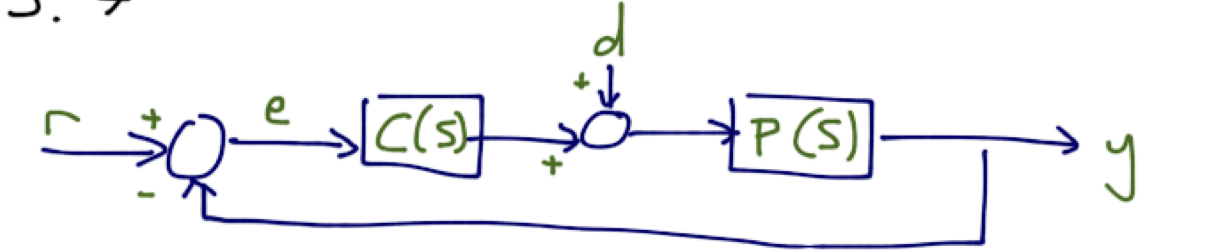
\includegraphics[width=0.5\textwidth,keepaspectratio]{images/5-7.png}\end{center}

                    \begin{align*}
                        P(s) &= \frac{1}{s^4 + 6s^3 + 11s^2 + 6s} \\
                        C(s) &= K
                    \end{align*}
                    Where $K$ is the real gain.

                    From section 5.1.1, we know that the feedback is stable iff all roots of $\Pi$ are in the left half complex plane.
                    \begin{align*}
                        \Pi(s) &= N_p N_c + D_p D_c \\
                        &= s^4 + 6s^3 + 11s^2 + 6s + K
                    \end{align*}

                    We know that k is gerater than 0 since... [missed this point.]

                    \begin{table}[h]
                        \centering
                        \begin{tabular}{ | l || l | l | l | l | }
                            \hline
                            \hline
                            $s^4$ & $1$ & $11$ & $k$ \\ \hline
                            $s^3$ & $6$ & $6$ & $0$ \\ \hline
                            $s^2$ & $\frac{66-6}{10} = 10$ & $\frac{6k - 0}{6} = k$ & $0$ \\ \hline
                            $s^1$ & $\frac{60-6K}{10} = \frac{3(10-k)}{5}$ & $0$& $0$\\ \hline
                            $s^0$ & $k$ & $0$& $0$\\ \hline
                        \end{tabular}
                    \end{table}

                    For feedback stability, we need all signs to be these same in the first column. $s^1 \to k < 10$, $s^0 \to k > 0$.

                    Thus, we know we should have $0 < k < 10$.
            \end{enumerate}

        \item 5.3 Steady state performance.

            \begin{center}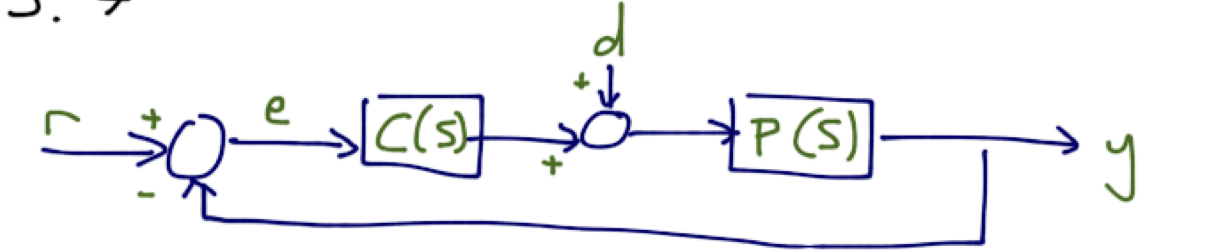
\includegraphics[width=0.5\textwidth,keepaspectratio]{images/5-7.png}\end{center}
            \begin{itemize}
                \item Closed-loop stability is essential
                \item Good performance is desirable, and can be measured as follows.
                    \begin{itemize}
                        \item Transient response ($T_s$, $\% OS$, etc)

                            Easy to measure for second order systems, but is hard to do in general.

                        \item Steady state.
                            \begin{itemize}
                                \item steady-state gain
                                \item tracking error
                                \item disturbance rejection
                            \end{itemize}
                            All of these are calculated using the final value theorem (FVT)
                    \end{itemize}
            \end{itemize}
            \begin{center}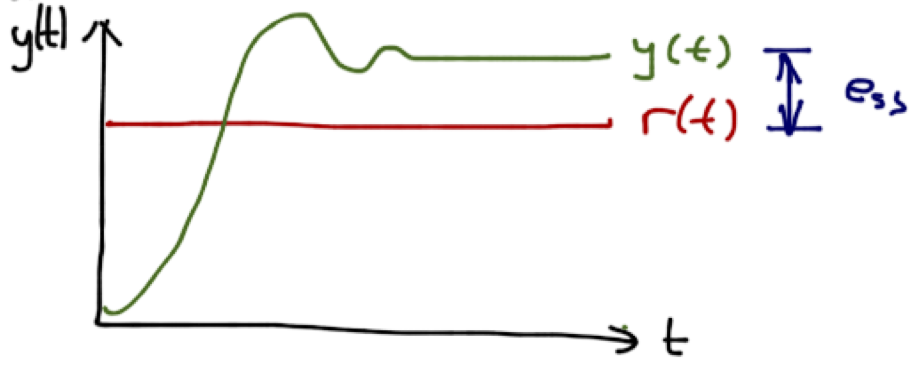
\includegraphics[width=0.5\textwidth,keepaspectratio]{images/5-10-a.png}\end{center}

            \begin{itemize}
                \item Example:
                    Cruise control regulates a car's speed to a desired (constant) value.
                    The principle behind its operation is The Final value theorem.
                    Car model:
                    \begin{align*}
                        \dx &= -x + u \\
                        &\Rightarrow \frac{Y(s)}{U(s)} = P(s) = \frac{1}{s+1} \\
                        y &= x
                    \end{align*}
                    If we take the integrator as our controller, we have:
                    \begin{align*}
                        u(t) &= \int_0^{\infty} e(\tau)d\tau \\
                        & \Rightarrow C(s) = \frac{1}{s}
                    \end{align*}
                    Since $\Pi(s) = s^2 + s + 1$, the feedback is stable (both poles are in the LHP)

                    Suppose the driver suddently changes the desired speed to $r_0$ (constant).
                    We can model this as a step chage ($r(t) = r_0$, $t \ge 0$)

                \item Steady-state tracking error:

                    TF from $R \to E = \frac{1}{1+PC} = \frac{D_p D_c}{N_p N_c + D_p D_c}$

                    Plugging in, we get:
                    \begin{align*}
                        E(s) &= \frac{s(s+1)}{s^2 + s + 1} \frac{r_0}{s}
                    \end{align*}

                    Since $\Pi$ is stable, the FVT applies:
                    \begin{align*}
                        e_{ss} \lim_{t \to \infty} e(t) &= \lim_{s \to 0} s E(s) \\
                        &= \lim_{s \to 0} s\frac{s(s+1)}{s^2 + s + 1} \frac{r_0}{s} \\
                        &= 0
                    \end{align*}

                    So the system provides \uline{perfect asymptotic tracking} of any step reference input.
                \item Why does this work?
                    \begin{enumerate}
                        \item In the frequency domain,
                            \begin{align*}
                                \frac{E(s)}{R(s)} &= \frac{1}{1+C(s)P(s)} \\
                            \end{align*}
                            As $\omega \to 0$, we get:
                            \begin{align*}
                                \frac{E(j \omega)}{R(j \omega)} &\to  \frac{1}{1+\infty}
                            \end{align*}
                            \begin{center}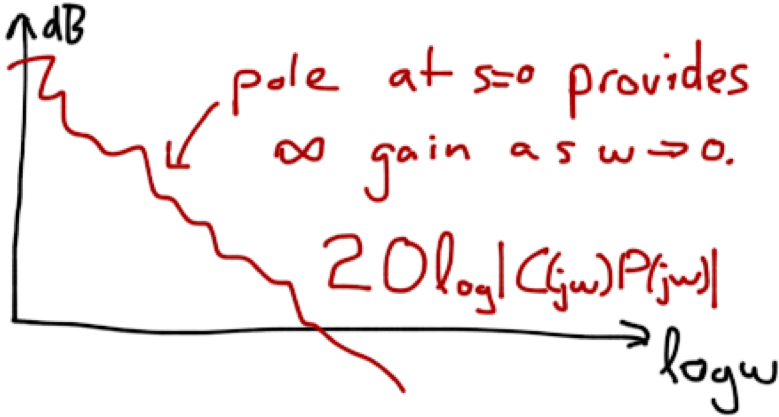
\includegraphics[width=0.5\textwidth,keepaspectratio]{images/5-11-a.png}\end{center}
                        \item In the time domain

                            \begin{center}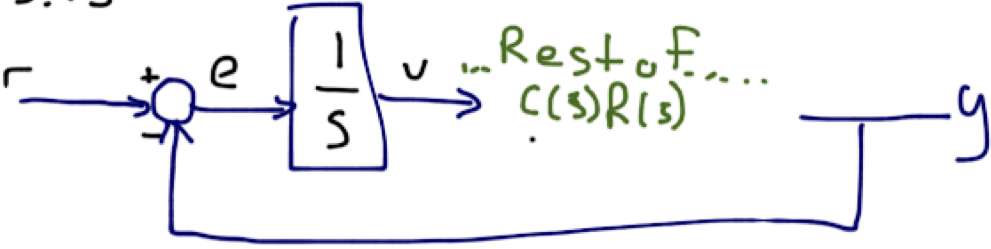
\includegraphics[width=0.5\textwidth,keepaspectratio]{images/5-11-b.png}\end{center}

                            If CLS is stable, all signals approach a constant as $t \to \infty$.
                            \begin{align*}
                                v(t) &= \int_0^t{e(\tau)d\tau} \\
                                \dot{v} &= e
                            \end{align*}
                            Since $v(t)$ approaches a constant, $e$ must go to zero
                        \item Internal Model Principle

                            The product $C(s)P(s)$ has a model of $R(s)$ (i.e. an integrator) embedded in it. Closing the loop creates a zero in the TF from $R$ to $E$ to exactly cancel the unstable part of $R(s)$.
                                Not an illegal cancellation, since we are cancelling a pole in the signal, not in the system.

                            Only the unstable parts of $R$ are the ones that we need to do tracking for, the other ones all go to a constant.
                    \end{enumerate}
                    In general, if $C(s)$ provides closed-loop stability, then FVT applies, and:
                    \begin{align*}
                        e_{ss} &= \lim_{t\to \infty} e(t) \\
                        &= \lim{s \to 0} s E(s) \\
                        &= \lim{s \to 0} s \frac{1}{1+ C(s)P(s)} \frac{r_0}{s} \\
                        &= \frac{r_0}{1+ C(0) P(0)}
                    \end{align*}
                    Therefore, we can say these are identical statements:
                    \begin{itemize}
                        \item $e_{ss} = 0$
                        \item $P(0) C(0) = \infty$
                        \item $P(s)C(s)$ has a pole at $s = 0$
                        \item $P(s)C(s)$ has at least one integrator.
                    \end{itemize}
                    So the integral control is fundamental for perfect step tracking.
                \item If $P(s)$ does not have a pole at $s = 0$ and we want perfect step tracking, the controller must be the one that provides the integration. Thus, it is common to pick:
                    \begin{align*}
                        C(s) = \frac{1}{s}C_1(s)
                    \end{align*}
                    so that $C(s)P(s)$ has an integrator. Then $C_1(s)$ is designed to stabilize the overall system.
                    \begin{center}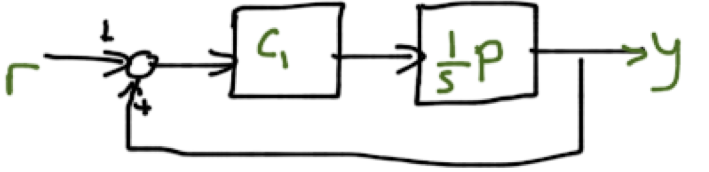
\includegraphics[width=0.5\textwidth,keepaspectratio]{images/5-11-c.png}\end{center}

                    The integrator decreases the phase plot of $P(s)$ which makes it harder to design $C_1$ to stabilize the whole system. There's no free lunch (as usual).
                    \begin{itemize}
                        \item If $C(0)P(0)$ is \uline{finite}, then the system $C(s)P(s)$ is called a \uline{type-0 system}, and $K_d := C(0)P(0)$ is the \uline{position error constant}.
                            \begin{align*}
                                e_{ss} &= \frac{r_0}{1 + K_p}
                            \end{align*}
                    \end{itemize}
                \item Example: Nonconstant Reference:

                    \begin{align*}
                        C(s) &= \frac{1}{s} \\
                        P(s) &= \frac{2s + 1}{s(s+1)} \\
                        E(s) &= \frac{1}{1+C(s)P(s)} R(s) \\
                        &= \frac{D_p D_c}{N_p N_c + D_p D_c} \frac{r_0}{s^2} \\
                        &= \frac{s+1}{s^3 + s^2 + 2s + 1}
                    \end{align*}

                    \begin{table}[h]
                        \centering
                        \begin{tabular}{ | l || l | l | l | l | }
                            \hline
                            \hline
                            $s^3$ & $1$ & $2$ & $0$ \\ \hline
                            $s^2$ & $1$ & $1$ & $0$ \\ \hline
                            $s^1$ & $1$ & $0$ & $0$ \\ \hline
                            $s^0$ & $1$ & $0$ & $0$ \\ \hline
                        \end{tabular}
                    \end{table}
                    Since the first column is the same sign, then $\Pi(s)$ is stable, and the feedback is stable.
            \end{itemize}
        \item 5.4 Intro to PID control.

            \begin{itemize}
                \item Majority of controllers in industry are Proportional-Integral-Derivative control.
                \item They are popular because:
                    \begin{itemize}
                         \item they are easy to tune
                         \item structure doesn't depent on plant model
                         \item often provides decent performance
                     \end{itemize}
            \end{itemize}

            Diagram of PID controllers:

            \begin{center}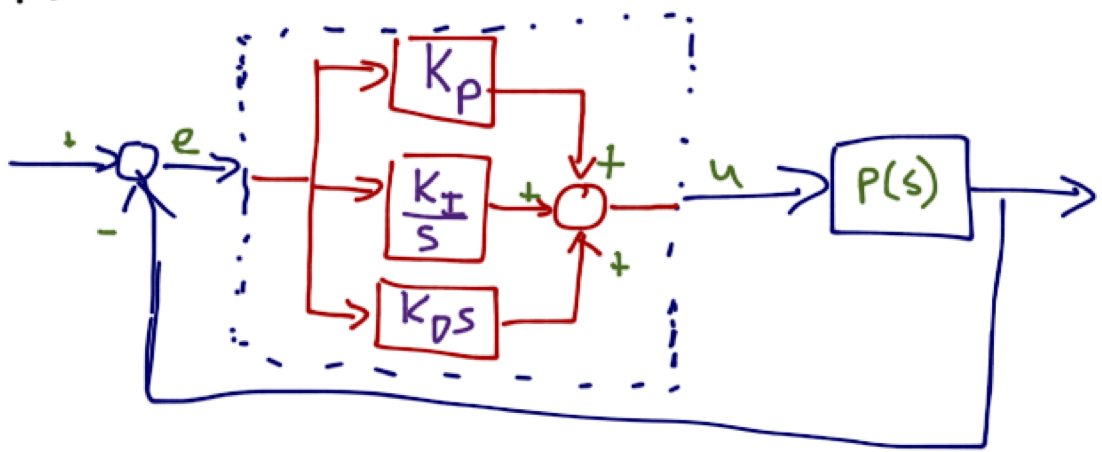
\includegraphics[width=0.5\textwidth,keepaspectratio]{images/5-8.png}\end{center}

            From this, we get:
            \begin{align*}
                C(s)&= K_p + \frac{K_i}{s} + K_d s \\
                    &= \frac{K_d s^2 + K_p s + K_i}{s} \\
                u(t) &= K_p e(t) + K_i \int_0^{\infty} {(e(\tau) d\tau)} + K_d \frac{de}{dt}
            \end{align*}

            The gains $K_d$, $K_i$, $K_D$ can be ``designed'' in the time or frequency domains. We see this in chapter 7.

            \begin{enumerate}
                \item Refinements to basic PIDs:
                    \begin{enumerate}
                        \item The basic PID is improper so it can't be implemented in practice.
                            \begin{enumerate}
                                \item To fix this, the derivative is usually to make it proper as follows:
                                    \begin{align*}
                                        C(s) = K_p + \frac{K_i}{s} + K_D \frac{s}{(\tau s + 1)}
                                    \end{align*}
                                    Where $\tau>0$ and is small.
                                \item Another way to implement $C(s)$ is by adding a pole to the ``whole thing'':

                                    \begin{align*}
                                        C(s) &= \frac{K_D s^2 + K_p s + K_i}{s (\tau s + 1)}
                                    \end{align*}
                                    $\tau > 0$ is small. (Is a different tau than before.)
                            \end{enumerate}
                        \item The reference signal is often discontinuous (i.e. it steps). Differentiating steps result in nasty impulses in the control signal. To avoid this, PID is implemented as the following:

                            \begin{center}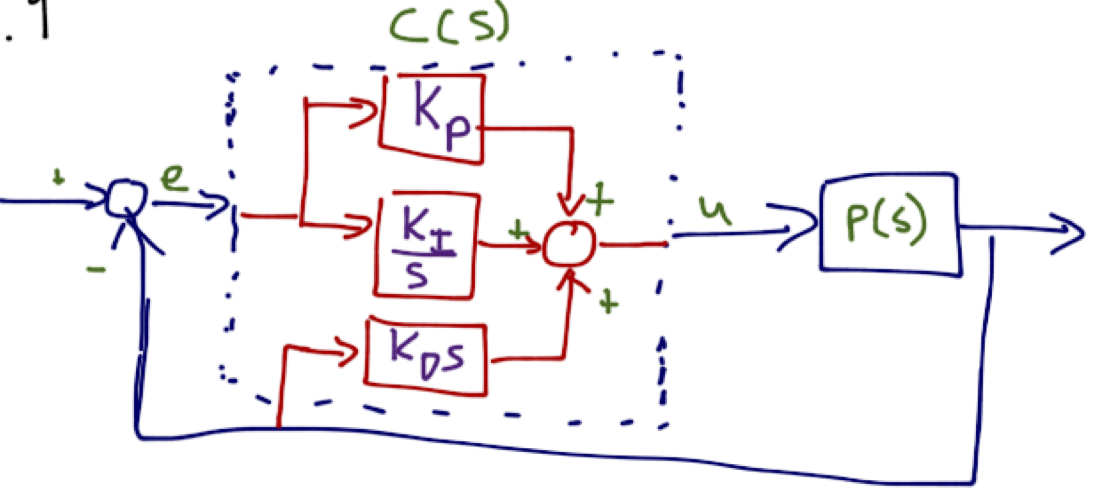
\includegraphics[width=0.5\textwidth,keepaspectratio]{images/5-9.png}\end{center}

                            Note: (TODO: move this to the correct location) $e_{ss} = r - y$.
                    \end{enumerate}
            \end{enumerate}
        \item Tracking ramps:
            \begin{align*}
                E(s) &= \frac{1}{P(s)C(s)} \frac{r_0}{s^2} \\
                &= \frac{D_p D_c}{N_p N_c + D_p D_c} \frac{r_0}{s^2}
            \end{align*}
            Think of partial fraction expansion. The signal $e(t)$ will blow up (like a ramp) unless one or both of the poles at $s = 0$ are cancelled.
            \begin{itemize}
                \item If $P(0)C(0)$ is finite, then $|e_{ss}| = \infty$
                \item If $P(s)C(s)$ has one or more poles at $s = 0$, and $C(s)$ provides CLS, then:
                    \begin{align*}
                        e_{ss} &= \lim_{t \to \infty}e(t) \\
                        &= \lim_{s \to 0} \frac{1}{P(s)C(s)} \frac{r_0}{s^2} \\
                        &= \frac{r_0}{s C(s)P(s)} |_{s=0}
                    \end{align*}
            \end{itemize}
            Therefore,
            \begin{align*}
                e_{ss} = 0 &\Leftrightarrow sC(s)P(s) |_{s=0} = \infty \\
                &\Leftrightarrow \text{There are \uline{at least} two integrators in PC}
            \end{align*}
            If $C(s)P(s)$ has one pole at $s = 0$ it's called a \uline{type-1} system, and the \uline{velocity error constant is}:
            \begin{align*}
                K_v &= s C(s)P(s)|_{s = 0}\\
                e_{ss} = \frac{r_0}{K_v}
            \end{align*}
            \begin{enumerate}
                \item Internal model principle:

                    If $P(s)$ is strictly proper, and $C(s)$ is proper and provides closed-lopp stability. If $C(s)P(s)$ contains a model of the unstable part of $R(s)$ then we get perfect asymptotic tracking.
                \item Example:
                    \begin{align*}
                        P(s) &= \frac{1}{s+1}
                    \end{align*}
                    Reference command: $r(t) = r_0 sin(t) \rightarrow R(s) = \frac{r_0}{s^2 + 1}$
                    Then $P(s)C(s)$ needs a model of the unstable parts of $R(s)$.

                    The unstable part of $R$ corresponds to poles at $s = \pm j$. Since $P$ does not have a pole at $s = j$ or $s = -j$, the controller must provide the internal model.

                    This suggests $C(s) = \frac{1}{s^2 + 1} C_1(s)$, i.e. embed the model in $C$ and design $C_1$ to achieve feedback stability.

                    In this case, $C_1(s) = s$ works.

                    Let's check:
                    \begin{align*}
                        \frac{E(s)}{R(s)} &= \frac{(s^2 + 1)(s+1)}{s^3 + s^2 + 2s + 1} \\
                        e_{ss} &= \lim_{s\to 0} s \frac{(s^2 + 1)(s+1)}{s^3 + s^2 + 2s + 1} \frac{r_0}{s^2 + 1} \\
                        &= 0
                    \end{align*}
                \item Steady-state disturbance rejection: [5.3.2]

                    \begin{center}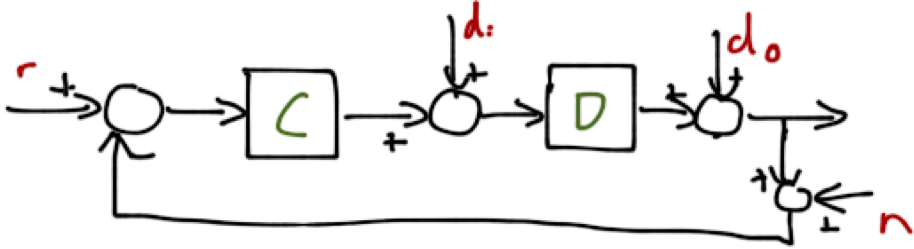
\includegraphics[width=0.5\textwidth,keepaspectratio]{images/5-12-a.png}\end{center}

                    Our \uline{Goal} is to minimize the effect of the disturbances and noise on the output $y$.

                    As before, we can use the final value theorem to analyze the effect of noise etc.

                \item Example:

                    Find conditions on $P$, $C$ so that the steady state effect of an output step disturbance is zero.

                    Use linearity to set $r = d_i = n = 0$

                    \begin{align*}
                        \frac{Y(s)}{D_0(s)} &= \frac{1}{1 + P(s)C(s)} \\
                        d_0(t) = d_{const}, t \ge 0.
                    \end{align*}
                    If $C(s)$ stabilizes the loop, then
                    \begin{align*}
                        y_{ss} &= \lim_{t\to \infty}y(t) \\
                        &= \lim_{s \to 0} s \frac{1}{1+PC} \frac{d_0}{s} \\
                        &= \frac{d_0}{1 + C(0)P(0)}
                    \end{align*}
                    Therefore $y_{ss} = 0 \Leftrightarrow $ PC has a pole at $s = 0$.
                \item Example (broomstick):

                    It's not always possible to track perfectly and get stability.

                    If you have an inverted pendulum on your hand as so: (i.e. a broomstick)

                    \begin{center}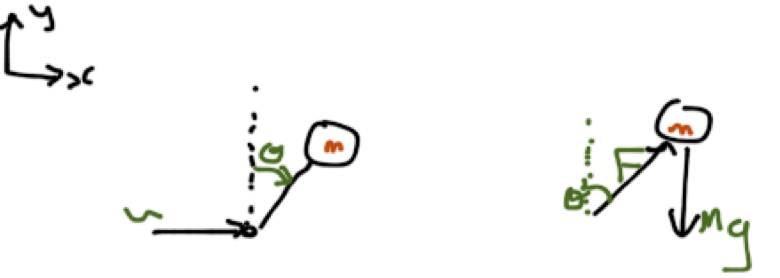
\includegraphics[width=0.5\textwidth,keepaspectratio]{images/5-12-b.png}\end{center}

                    Horizontal position: $u + L \sin{\theta}$

                    Vertical position: $L \cos{\theta}$

                    Horizontal equation of motion:
                    \begin{align*}
                        m \frac{d^2}{dt^2} (\text{Horizontal position}) &= F \sin{\theta}
                    \end{align*}
                    Vertical equation of motion:
                    \begin{align*}
                        m \frac{d^2}{dt^2} (\text{Vertical position}) &= F \cos{\theta} - mg
                    \end{align*}
                    We can take the linear approximation by assuming that if $\theta$ is small mass only moves in the horizontal direction:
                    Horizontal:
                    \begin{align*}
                        m \dot{u} + m L \ddot{\theta} &= F\theta
                    \end{align*}
                    Vertical:
                    \begin{align*}
                        0 &= F - mg \\
                        \rightarrow \dot{u} + L\ddot{\theta} &= g \theta \\
                        \rightarrow s^2 U(s) + s^2 L \Theta(s) &= g \Theta(s) \\
                        \frac{\Theta(s)}{U(s)} &= \frac{-s^2}{Ls^2 - g} \\
                        &= P(s)
                    \end{align*}
                    $P(s)$ has zeros at $s = 0$, so we can't pick $C(s) = \frac{1}{s} C_1(s)$, so we can't embed an internal model if $R(s) = \frac{r_0}{s}$ without adding an unstable pole-zero cacellation.

                    Perfect tracking and internal stability are not possible.
            \end{enumerate}

    \item Loopshaping - High-gain control revisited: [5.12]
        \begin{enumerate}
            \item Key Idea:

                the choice of high-gain versus low-gain is a \uline{frequency-dependent choice}:

                \begin{center}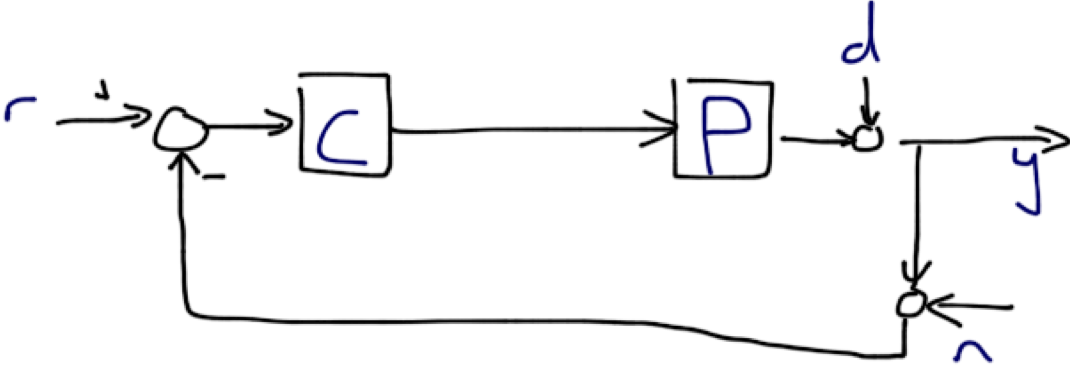
\includegraphics[width=0.5\textwidth,keepaspectratio]{images/5-13-a.png}\end{center}

                So,
                \begin{align*}
                    Y(s) &= \frac{PC}{1+PC} R(s)  + \frac{1}{1+PC}D(s) - \frac{PC}{1+PC} N(s) \\
                \end{align*}
                \begin{itemize}
                    \item To minimize the effect of $d$ on $y$ at frequency $\omega$, $|P(j\omega) C(j\omega)|$ should be \uline{large}
                    \item To have the TF from $r$ to $y$ close to one at a frequency $\omega$, we need $|P(j\omega) C(j\omega)|$ to be \uline{large} (again)
                    \item To minimize the effect of noise at frequency $\omega$ we need $|P(j\omega) C(j\omega)|$ to be \uline{small}.
                \end{itemize}

            \item Rule of thumb (overview):

                Use high gain at frequencies where tracking/disturbance rejection is required. Use low gain at frequencies where noise is active.

                At intermediate frequencies, we will do whatever it takes to stabilize the closed-loop system.
                \begin{center}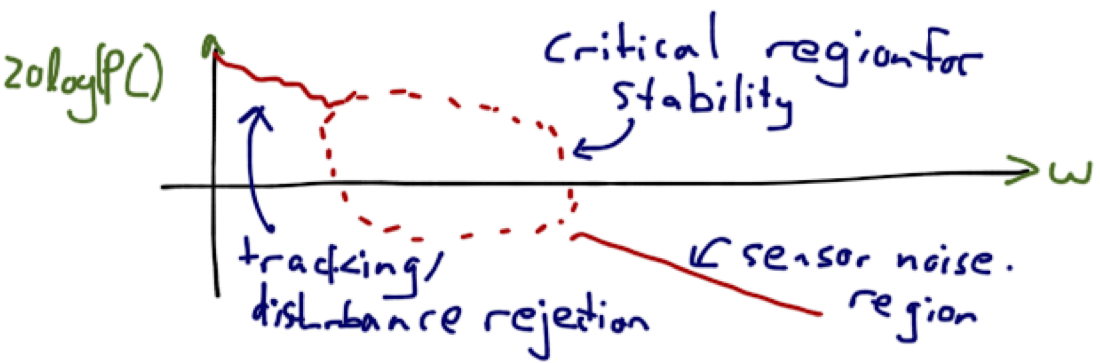
\includegraphics[width=0.5\textwidth,keepaspectratio]{images/5-13-b.png}\end{center}
        \end{enumerate}
    \item Root Locus Methods [Chapter 6]
        \begin{enumerate}
            \item Loop shaping gives us intuition about our gain choices.
            \item Root Locus gives us a picture of how closed-loop poles $\Pi(s) = D(s) + KN(s)$ moves as a single parameter varied.
            \item Root Locus Methods
                \begin{center}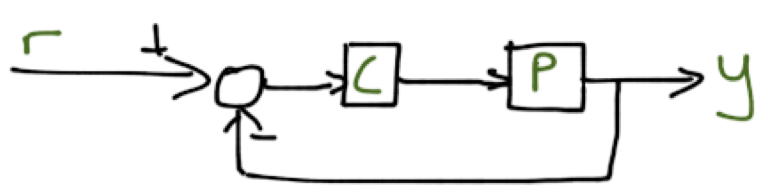
\includegraphics[width=0.5\textwidth,keepaspectratio]{images/6-1-a.png}\end{center}
                \begin{align*}
                    \Pi(s) &= N_c N_p + D_c D_p
                \end{align*}
                \begin{itemize}
                    \item Closed loop poles (roots of $\Pi$) determine stability directly and indirectly performance.
                    \item If $\Pi$ has uncertain plant parameters or controller gains, we can use Routh-Hurwitz to determine stability but not much else.
                    \item Root-locus gives much more info:
                        \begin{itemize}
                            \item Shows how poles move on the $s$-plane as a single parameter is varied
                            \item Ease of use makes it an efficient analysis tool
                            \item Can be used (for limited) design
                            \item In matlab, we use the #rltool# command.
                        \end{itemize}
                \end{itemize}


            \item Example:
                \begin{align*}
                    C(s) &= K \\
                    P(s) &= \frac{1}{s(s+2)} \\
                    \Pi(s) &= s^2 + 2s + K \\
                    \text{Closed-loop poles: }s &= -1 \pm \sqrt{1 - K}
                \end{align*}
                \begin{center}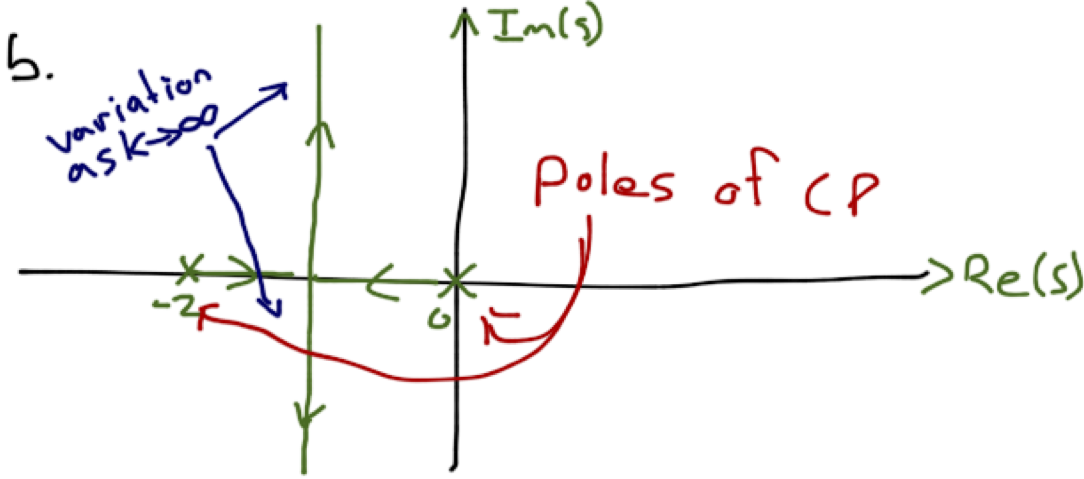
\includegraphics[width=0.5\textwidth,keepaspectratio]{images/6-1-b.png}\end{center}
                \begin{enumerate}
                    \item $K< 0$, unstable
                    \item $K = 0$ poles at $s = 0$, $s = -2$, unstable
                    \item $K \in (0, 1)$ two real distinct \& stable poles
                    \item $K = 1$ two real repeated \& stable poles
                    \item $K > 1$ complex conjugate roots, with real part $= -1$
                \end{enumerate}

            \item Basic construction of the Root-locus: [Chapter 6.1]

                Consider a unity-feedback system with a gain pulled out of the controller:

                \begin{center}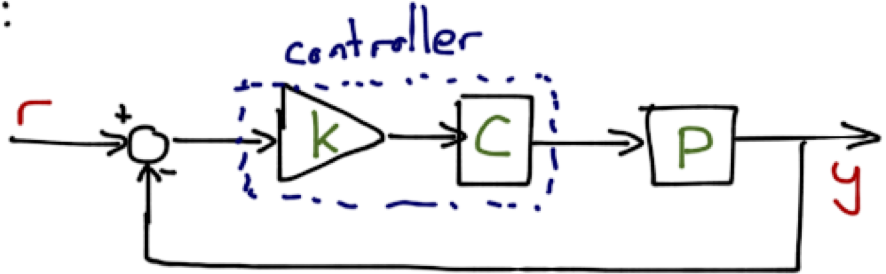
\includegraphics[width=0.5\textwidth,keepaspectratio]{images/6-1-c.png}\end{center}
                \begin{align*}
                    \frac{Y(s)}{R(s)} &= \frac{K C(s)P(s)}{1 + K C(s) P(s)} \\
                    &= \frac{K N(s)}{K N(s) + D(s)} \\
                    \Pi(s) &= D(s) + K N(s)
                \end{align*}
                We write $C(s)P(s) = \frac{N(s)}{D(s)}$, $n := \deg(D(s))$, $m := \deg(N(s))$
            \item Root-locus assumptions:

                We are given two polynomials $N(s)$ and $D(s)$, and want to show graphically how the roots of $\Pi$ vary with the scalar $K$.

                We make the assumption that:
                \begin{itemize}
                    \item $n \ge m$ (i.e. $C(s)D(s)$ is proper)
                    \item $K$ varies from $ 0 \to \infty$
                    \item $N(s)$ and $D(s)$ are monic (leading coefficients are $1$).
                \end{itemize}
            \item Construction rules:
                \begin{itemize}
                    \item The Root-locus is symmetric about the real axis.

                        Since $\Pi$ has real coefficients

                    \item The Root-locus consists of $n$ \uline{branches}

                        Since $\Pi$ is of $n^{th}$ order, it has $n$ roots (which become branches, apparently)

                    \item The Root-locus is a continuous function of $K$.

                    \item The root locus ``start'' (i.e. $K = 0$) at the roots of $D(s)$

                        When $K = 0$, $\Pi(s) = KN(s) + D(s) = D(s)$, i.e. the open-loop poles.

                    \item As $K \to \infty$, $m$ of the branches will terminate at the roots of $N(s)$

                        The roots of $N(s)$ are the zeros of $C(s)P(s)$
                        This is not immediately obvious.

                        The remaining $n-m$ branches go to infinity along asymptotes.

                        The $i^{\text{th}}$ asymptote has the angle $\phi _i$:

                        \begin{align*}
                            \phi_i &= \frac{(2+i)\pi}{n-m} \text{, } i\in \mathbbold{N}
                        \end{align*}

                        and intersects the real axis at a \uline{centroid}:

                        \begin{align*}
                            \sigma &= \frac{\Sigma{(\text{roots of }D(s))} - \Sigma{(\text{roots of} N(s))}}{n-m}
                        \end{align*}

                        \begin{center}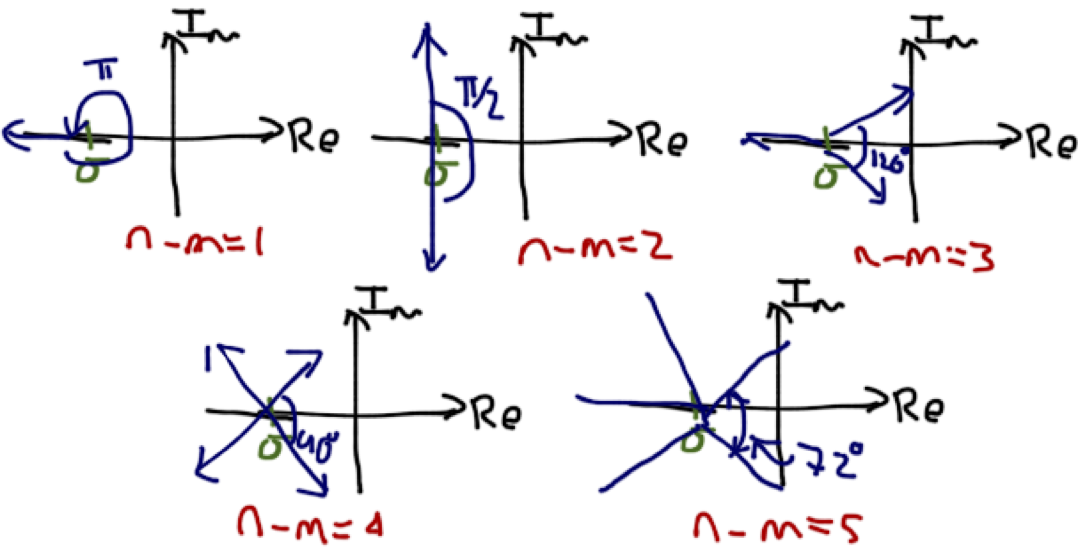
\includegraphics[width=0.5\textwidth,keepaspectratio]{images/6-2-a.png}\end{center}

                    \item (``no-yes-no'' rule) A point $s$ on the real axis is part of the root locus if and only if the total number of poles and zeros of $\frac{N(s)}{D(s)}$ to the right of $s$ is \uline{odd}.

                        \begin{center}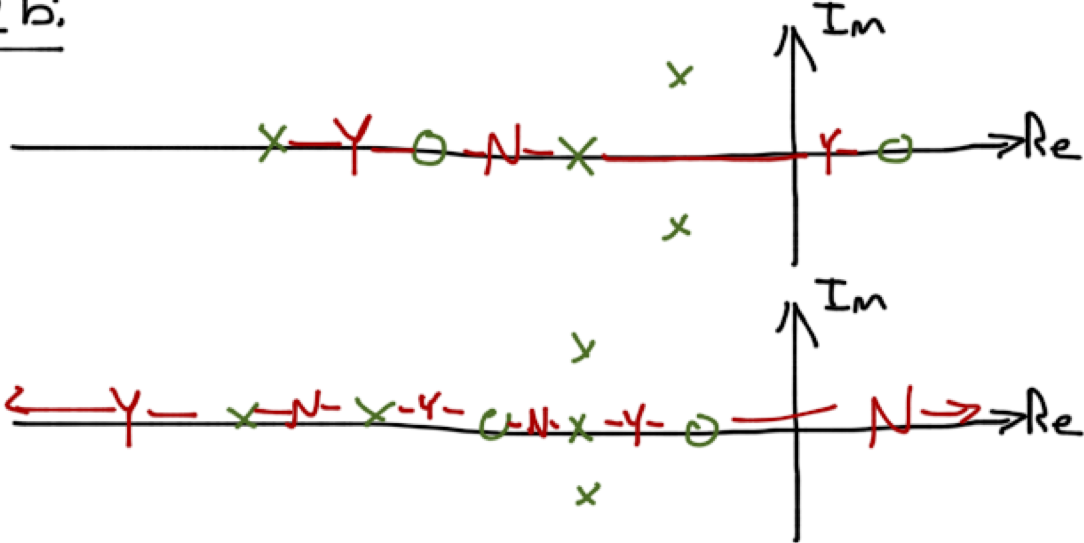
\includegraphics[width=0.5\textwidth,keepaspectratio]{images/6-2-b.png}\end{center}

                    \item Example:

                        \begin{center}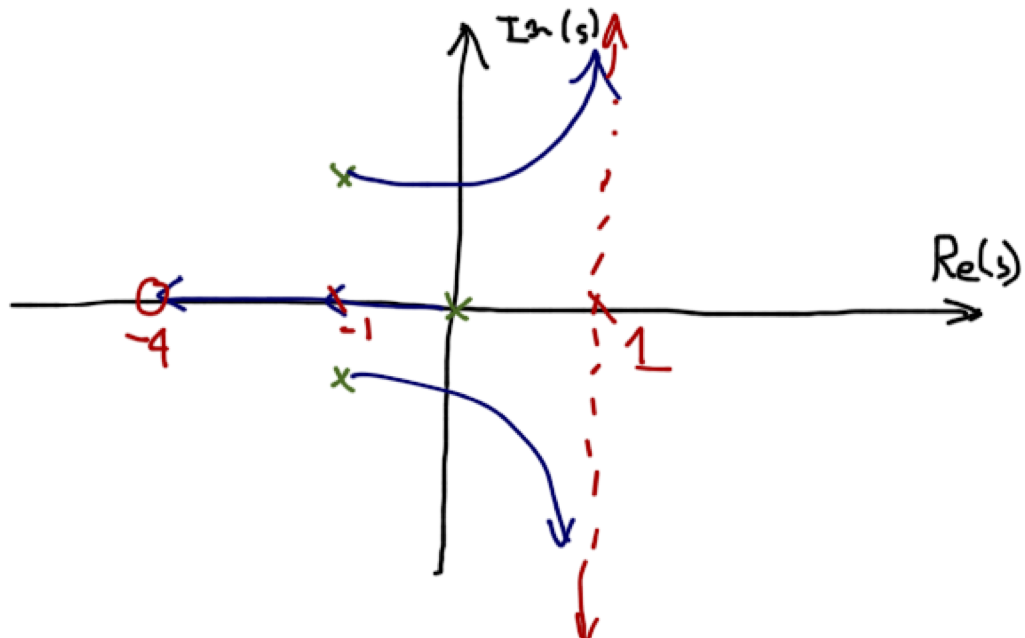
\includegraphics[width=0.5\textwidth,keepaspectratio]{images/6-2-c.png}\end{center}
                        \begin{align*}
                            N(s) &= s + 4 \\
                            \rightarrow m &= 1 \\
                            D(s) &= s(s^2 + 2s + 5) \\
                            \rightarrow n &= 3 \\
                            \Pi(s) &= KN(s) + D(s) \\
                        \end{align*}

                        \begin{enumerate}
                            \item Plot zeros (roots of $N$) and poles (roots of $D$)
                            \item Use ``no-yes-no'' rele to fill in the real axis
                            \item Find asymptotes

                                \begin{align*}
                                    \sigma &= \frac{\Sigma{(\text{roots of }D(s))} - \Sigma{(\text{roots of} N(s))}}{n-m} \\
                                    &= \frac{0 + (-1+2j) + (-1-2j) + (-4)}{3-1}
                                \end{align*}

                            \item Sketch \uline{rough} root locus ($rule 5$) implies the pole at $s = 0$ moves towards zero at $s = -4$
                            \item We could use RH to determine when the RL crosses imaginary axis
                        \end{enumerate}

                    \item Example:
                        \begin{align*}
                            \Pi(s) &= s^3 (s+4) + K(s+1) \\
                            D(s) &= s^3 (s+4) \\
                            \rightarrow n &= 4 \\
                            N(s) &= K(s+1) \\
                            \rightarrow m &= 1 \\
                            \rightarrow \sigma &= -1
                        \end{align*}

                        \begin{center}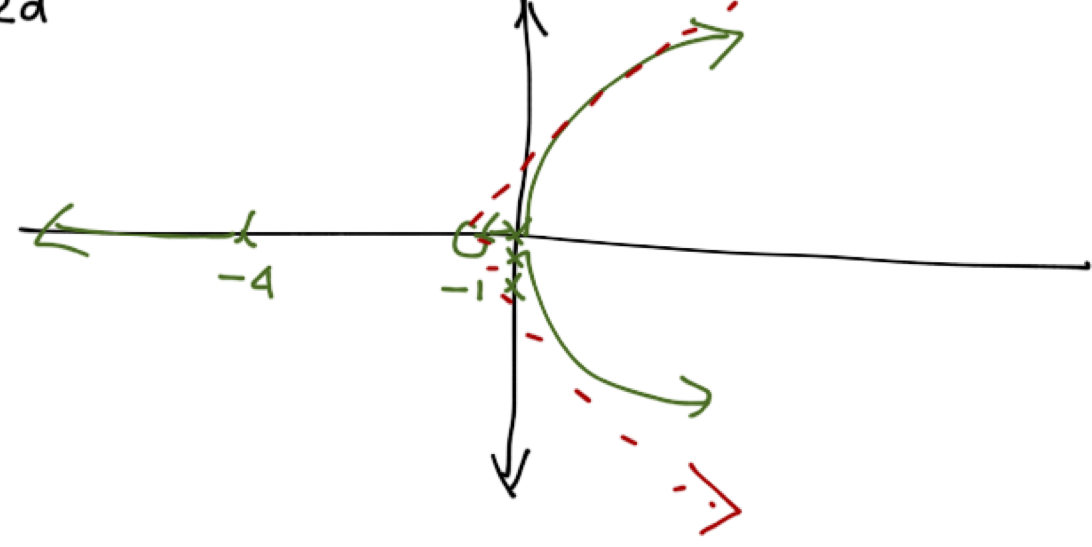
\includegraphics[width=0.5\textwidth,keepaspectratio]{images/6-2-d.png}\end{center}
                    \item Example:

                        \begin{center}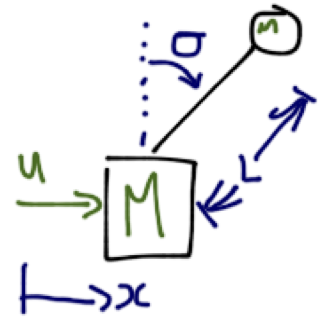
\includegraphics{images/6-2-e.png}\end{center}

                        \begin{center}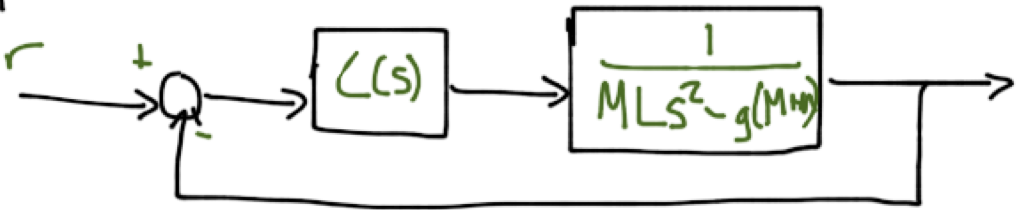
\includegraphics[width=0.5\textwidth,keepaspectratio]{images/6-2-f.png}\end{center}

                        Determine how closed-loop poles vary as a function of $k$ for a $P$, $PD$, $PI$, and $PID$ controller.
                        \begin{itemize}
                            \item $P$ Controller:

                                \begin{align*}
                                    C(s) &= K \\
                                    \Pi(s) &= MLs^2 - g(M+m) + K \\
                                    D(s) &= MLs^2 - g(M+m) \\
                                    n &= 2 \\
                                    N(s) &= 1 \\
                                    m &= 0
                                \end{align*}

                                $P$ cannot stabilize

                            \item $PD$ controller:
                                \begin{align*}
                                    C(s) &= K_p + K_D s \\
                                    &= K(1 + \tau s) \\
                                    \Pi(s) &= MLs^2 - g(M+m) + K (1+\tau s) \\
                                    D(s) &= MLs^2 - g(M+m) \\
                                    N(s) &= (1+\tau s)
                                \end{align*}
                        \end{itemize}
                    \item Summary:
                        \begin{itemize}
                            \item Root locus gives us a picture of how closed-loop poles move wrt a single changing variable.
                            \item Basic rules (1-6) operate on the asymptotes and centroids.
                            \item We went through an example using Root-locus to decide on a controller type.
                        \end{itemize}
                \end{itemize}
            \item Example:

                TODO: insert Diagram 6-13a.

                \begin{align*}
                    P(s) &= \frac{1}{M\ell s^2 - g(m+M)}
                \end{align*}
                This is connnected in unity-feedback
                \begin{align*}
                    C(s) &= {P, PD, PI, PID}
                \end{align*}
                \begin{enumerate}
                    \item P cannot stabilize (from last class.) TODO: coagulate
                    \item PD:
                        \begin{align*}
                            C(s) &= K_p K_D s \\
                            &= K(1 + \tau s)
                        \end{align*}
                        TODO: insert Diagram 6-13b
                    \item PI:
                        \begin{align*}
                            C(s) &= K_P + \frac{K_I}{s} \\
                            &= K(1+\frac{a}{s}) \\
                            &= K (\frac{s+a}{s}) \\
                            \Pi(s) &= s(M\ell s^2 - g (M+m)) + K(s+a) \\
                            \rightarrow D(s) &= s(M\ell s^2 - g (M+m)) \\
                            \rightarrow N(s) &= K(s+a)
                        \end{align*}
                        TODO: insert Diagram 6-13c
                    \item PID
                        \begin{align*}
                            C(s) &= K_P + \frac{K_I}{s} + K_D s \\
                            &= K(a + \frac{b}{s} + s) \\
                            &= K \frac{s^2 + as + b}{s} \\
                            \Pi(s) &= s (MLs^2 - g(m+M)) + K(s^2 + as + b) \\
                            \rightarrow D(s) &= (MLs^2 - g(m+M)) \\
                            \rightarrow R(s) &= (s^2 + as + b)
                        \end{align*}
                        TODO: insert Diagram 6-13d
                \end{enumerate}
            \item Rules $7 \to 9$: Refer to notes. He doesn't care about these. [Chapter 6.2]
        \end{enumerate}
    \item Non-Standard Problems: [6.3]

        We made 3 major assumptions in the basic root locus constructions:
        \begin{itemize}
            \item Unity Feedback
            \item We can ``pull'' a gain out of $C(s)$
            \item $\Pi(s) D(s) + K N(s)$, $\deg(D) \ge \deg(N)$
        \end{itemize}
        Here's how you tackle these problems:
        \begin{enumerate}
            \item Sensor dynamics:

                TODO: insert diagram 6-13e

                Let:
                \begin{align*}
                    \frac{N(s)}{D(s)} &= C(s) P(s) H(s)\\
                    \rightarrow \Pi(s) &= KN(s) + D(s)
                \end{align*}

                In other words, the RL is exactly the same, except:
                \begin{align*}
                    N(s) &= N_c N_p N_h \\
                    D(s) &= D_c D_p D_h
                \end{align*}
            \item Non-fixed parameter can't be factored from controller:

                Even if $K$ can't be factored from $C(s)$, the characteristic polynomial will still have the form
                $\Pi(s) = KN(s) + D(s)$ but in this case, $D(s) \ne D_c D_p$, $N(s) \ne N_c N_p$

                \begin{itemize}
                    \item Example:

                        TODO: insert diagram 6-13f

                        PD Controller $C(s) = 10 (1+ \tau s)$, can't factor $\tau$ out.

                        \begin{align*}
                            \Pi(s) &= s(s+2) + 10 (1 + \tau s)\\
                            &= (s^2 + 2s + 10) + (10\tau) s\\
                            \rightarrow D(s) &= (s^2 + 2s + 10)\\
                            \rightarrow K &= (10\tau) \\
                            \rightarrow N(s) &= s
                        \end{align*}

                        TODO: insert diagram 6-13g
                \end{itemize}

            \item Deg(D) < Deg(N)

                \begin{align*}
                    \Pi(s) &= D(s) + K N(s) \\
                    &= 0 \\
                    \Longleftrightarrow N(s) + \frac{D(s)}{K} &= 0
                \end{align*}
                Define the following:
                \begin{align*}
                    \hat{D} &= N \\
                    \hat{N} &= D \\
                    \hat{K} &= \frac{1}{K}
                \end{align*}
                We can draw the root locus for:
                \begin{align*}
                    \hat{\Pi}(s) &= \hat{D} + \hat{K} \hat{N} \\
                    \hat{K} : 0 \to \infty
                \end{align*}
                We will need to reverse everything, including the root locus, etc.
                \begin{itemize}
                    \item Example:
                        \begin{align*}
                            C(s) &= \frac{s+3}{\tau s + 1} \\
                            P(s) &= \frac{1}{s(s+1)}
                            \Pi(s) = (s+3) + (\tau s + 1) (s(s+1)) \\
                            &= expand
                            \hat{D} &= s^2 (s+1) \\
                            \hat{N} &= s^2 + 2s + 3 \\
                            \hat{K} &= 1/\tau
                            \hat{n} = 3 \\
                            \hat{m} &= 2 \\
                        \end{align*}
                    TODO: insert diagram 6-13h

                \end{itemize}
            \item Summary:
                \begin{enumerate}
                    \item Use RL to pick a controller:
                    \item Non-standard RL problems
                        \begin{enumerate}
                            \item $\text{deg}(D) < \text{deg}(N)$

                                \begin{align*}
                                    \Pi(s) &= D(s) + KN(s)
                                \end{align*}
                            \item Example:
                                \begin{align*}
                                    \Pi(s) &= s^2 + 2s + 3 + \tau s^2 (s + 1) \\
                                    \rightarrow_{\tau \to \infty} \tau s^2 (s + 1)
                                \end{align*}
                                TODO: insert diagram 6-14a
                        \end{enumerate}
                \end{enumerate}
        \end{enumerate}
    \item Introduction to control design [Ch. 7]
        \begin{itemize}
            \item ``classical'' conrol design
                \begin{enumerate}
                    \item lead
                    \item lag
                    \item lead-lag
                \end{enumerate}
            \item specs are in terms of bandwidth and \uline{stability margins}
            \item Our real interest is how the system behaves in physical time in using freq domain. We'll employ the duality between frequency and time.
            \item Design Philosophy:
                \begin{enumerate}
                    \item Take time domain specs and convert into frequency domain.
                        \begin{align*}
                            \begin{bmatrix}
                                \text{\% OS} \\
                                T_s \\
                                \text{tracking}
                            \end{bmatrix}
                            &\rightarrow
                            \begin{bmatrix}
                                \text{BW} \\
                                \text{gain margin} \\
                                \text{phase margin}
                            \end{bmatrix}
                        \end{align*}

                    \item Adjust gains to meet steady-state specs
                    \item Design a dynamic controller (TF) to meet other specs without affecting the gains too much.
                    \item Simulate a controller
                    \item If necessary, adjust specs and restart.
                \end{enumerate}
        \end{itemize}
        \begin{enumerate}
            \item Inro to stability margins [7.1]:

                If a system is stable, how stable is it?
                This depends entirely on our plant model, how we get it, and what uncertainty there is about the model.

                In the frequency domain, uncertainty is naturally measured in terms of gain and phase as functions of frequency.

                To understand stability margins, we need the Nyquist stability critereon.
                Instead, for now, we'll find stability margins from the Bode plot.
                \begin{itemize}
                    \item Gain margin: ($G_M$)

                        TODO: insert diagram 6-14b

                        Think $k = 1$ as our \uline{normal model} (gain margin $G_M$).

                        \begin{align*}
                            G_M = \sup\{\overline{k} \ge 1 : \text{closed-loop stability for } k \in [1, \overline{k}) \}
                        \end{align*}
                    \item Phase margin: ($P_M$)

                        TODO: insert diagram 6-14c

                        Think of $\phi = 0$ as the \uline{nominal model} (phase model $P_M$)

                        \begin{align*}
                            P_M = \sup\{ \overline{\phi} \ge 0 : \text{closed-loop stability for any } \phi \in [0, \overline{\phi}) \}
                        \end{align*}
                    \item Collectively, $P_M$ and $G_M$ are called the \uline{stability margins}.

                        Large stability margins not only imply robustness, but also good transient behaviour.

                        TODO: insert diagram 6-14d

                        Let $L(s)$ be as follows:

                        \begin{align*}
                            L(s) &= C(s)P(s)H(s)
                        \end{align*}
                        Draw the bode plot of $L(j \omega)$:

                        TODO: insert 6-14e
                    \item $\omega_{P_M}$
                        \begin{itemize}
                            \item Freq at which we measure $P_M$
                            \item called the \uline{gaincrossover frequency}
                            \item $\omega$ at which $20 \log{|L(j\omega)|} = 0$
                        \end{itemize}
                        \begin{align*}
                            P_M = 180 - \phase{L(j \omega_{P_M})}
                        \end{align*}
                    \item $\omega_{G_M}$
                        \begin{itemize}
                            \item freq at which we measure $G_M$
                            \item called the \uline{phase crossover frequency}
                            \item $\omega$ at which $\phase{L(j \omega)} = -180$
                        \end{itemize}
                        \begin{align*}
                            G_M = -20 \log{|L (j \omega_{G_M})|}
                        \end{align*}
                \end{itemize}

            \item Design Problem [7.2]
                \begin{itemize}
                    \item Given a plant $P(s)$ and a set of specs (common ones are closed-loop stability, transient stability, steady-state, $G_M$, $P_M$, bandwidth),
                        Design $C(s)$ so that closed-loop system meets the specs.

                        We focus on the following criteria:
                        \begin{enumerate}
                            \item Closed-loop stability
                            \item Tracking error
                            \item \% OS (Converted to $P_M$)
                            \item Bandwidth
                        \end{enumerate}

                        We focus on the following controllers:
                        \begin{enumerate}
                            \item Lag:
                                \begin{align*}
                                    C(s) &= K_c \frac{s+z}{s+p} \\
                                    z > p > 0
                                \end{align*}
                                TODO: insert diagram 6-14f
                            \item Lead:
                                \begin{align*}
                                    C(s) &= K_c \frac{s+z}{s+p} \\
                                    p > z > 0
                                \end{align*}
                                TODO: insert diagram 6-14g
                            \item Lead-lag:
                                \begin{align*}
                                    C(s) &= K_c \frac{s+z_1}{s+p_1}\frac{s+z_2}{s+p_2}
                                \end{align*}
                                Lucas W. posted a link to intuitively explain the Lead-Lag controller.
                                \href{http://en.wikipedia.org/wiki/Lead%E2%80%93lag_compensator#Intuitive_explanation}{Wiki Article}
                        \end{enumerate}
                        We focus on these because they are simple but useful. Also the are closely related to PID controllers.

                        The approch we'll discuss works well for ``nice plants''
                        \begin{enumerate}
                            \item stable or at worst one pole at $s = 0$
                            \item only one crossover frequency.
                        \end{enumerate}
                \end{itemize}
                \begin{enumerate}
                    \item Relationship between crossover frequency and bandwidth: [7.2.1]

                        \begin{align*}
                            \frac{Y(s)}{R(s)} &= \frac{C(s)P(s)}{1+C(s)P(s)} \\
                            &= T(s)
                        \end{align*}
                        TODO: Insert diagram 7-1a

                        Usually:
                        \begin{align*}
                            \omega_{P_M} < \omega_{BW} < \omega_{GM}
                        \end{align*}
                        For purposes in this course, we use:
                        \begin{align*}
                            \omega_{P_M} \approx \omega_{BW}
                        \end{align*}
                    \item Damping ratio and phase margin:

                        We claimed that small stability margins may mean por transient response.
                        This relationship can be quantified \uline{exactly} for 2nd order systems:

                        TODO: insert diagram 7-1b

                        i.e.
                        \begin{align*}
                            \frac{Y}{R} &= \frac{\omega_n^2}{s^2 + 2 \zeta \omega_n s + \omega_n^2}
                        \end{align*}

                        We can compute the $P_M$ exactly:
                        \begin{align*}
                            P_M &= atan\left[2 \zeta \sqrt{\sqrt{1 + 4 \zeta} - 2 \zeta ^2}\right]
                        \end{align*}

                        TODO: insert diagram 7-1c
                        \begin{align*}
                            \Rightarrow P_M &= 100 \zeta \\
                        \end{align*}
                        Where $P_M$ is measured in degrees, and $0 \le \zeta < 0.7$
                        \begin{itemize}
                            \item Example:

                                If we want our CLS to behave like a second order system with $\zeta = 0.65$, so we should make sure $P_M = 65\textdegree$
                        \end{itemize}
                \end{enumerate}

            \item Lag compensation: [7.3]

                TODO: insert diagram 7-1d

                \begin{align*}
                    C(s) &= K C_1(s)  \\
                    &= K \frac{\alpha Ts + 1}{Ts + 1} \\
                    0 < \alpha < 1 \\
                    T > 0 \\
                    K > 0
                \end{align*}
                We observe the following:
                \begin{itemize}
                    \item Log controller has DC gain $K$
                    \item Has a pole at $s = \frac{-1}{T}$ and zero at $s = \frac{-1}{\alpha T}$
                \end{itemize}

                TODO: insert diagram 7-1E

                The key benefit is high frequency gain reduction without affecting low frequency gain or high frequency phase as follows:

                TODO: insert diagram 7-1F

                Lag is used for two purposes:
                \begin{enumerate}
                    \item Boost the low frequency gain (and improve steady-state performance) without much effect on $G_M$, $P_M$, nor high frequency behavior.
                    \item To increase $P_M$ (at the cost of reducing the bandwidth)

                        TODO: insert diagram 7-1G
                \end{enumerate}

                \begin{itemize}
                    \item Example:

                        \begin{align*}
                            P(s) &= \frac{1}{s(s+2)}
                        \end{align*}

                        Specs:
                        \begin{enumerate}
                            \item $r(t) = r_0 t$, $t \ge 0$, $|e_{ss}| \le 0.05 r_0$
                            \item $P_M = 45 \textdegree$
                        \end{enumerate}

                        \begin{enumerate}
                            \item Choose K to meet the first spec:
                                \begin{align*}
                                    \lim_{t \to \infty}e(t) &= \lim_{s \to 0}s E(s) \\
                                    &= \lim_{s \to 0}s \left. \frac{r_0}{sC(s)P(s)} \right|_{s = 0} \\
                                    &= \frac{r_0}{K / 2} \\
                                    &\le 0.05 r_0 \\
                                    \rightarrow K &\ge \frac{2}{0.05} \\
                                    K &\ge 40
                                \end{align*}


                                We could've picked a bigger $K$, but we may as well do equal to $40$.

                                Pick $K = 40$
                            \item Draw bode of $KP(s) = \frac{40}{s(s+2)}$

                                From the plot, we get $\omega_{PM} = 6$ rad/s, $P_M = 18 \textdegree$

                                $\omega_{PM}$ is the gain crossover frequency.

                                To increase $P_M$ while preserving $K = 40$, we use a lag controller.

                                We'll actually aim for $P_M = 50 \textdegree$ to compensate for Bode approximation.

                                From Bode plot of $KP(s)$, we get:

                                \begin{align*}
                                    P_M^{\text{desired}} &= 45 + \delta \\
                                    &= 50\textdegree \\
                                    &= 180 \textdegree + \phase{KP(j \omega)}
                                \end{align*}

                                We choose $\delta = 5$ \textdegree because that's about how much the bode plot is off from 90\textdegree.

                                This works for when $\omega = 1.7$ rad/s

                                So we want to make the new gain crossover frequency equal to 1.7 rad/s without changing the phase at $\omega = 1.7$ rad/s

                                Tl;dr: we are trying to decrease the magnitude so it crosses zero at $\log(1.7)$ without changing the phase. In this example, that is a $19$ dB decrease.

                            \item Getting $\alpha$

                                From the Bode plot, we choose $20\log|KP| = 19dB$ at $\omega  = 17$ rad/s

                                So we want to reduce the gain by 19dB at $\omega = 1.7$ without changing the phase.

                                \begin{align*}
                                    20 \log \left| \frac{\alpha T j \omega + 1}{T j \omega + 1} \right|_{\omega = 1.7} &= -19 \\
                                    &= 20 \log \alpha \\
                                    \rightarrow \alpha &= 0.111
                                \end{align*}

                            \item Getting $T$:

                                $\phase{\frac{j\omega}{10} + 1}$ is the point where the phase angle meets the axis.

                                Set $\frac{10}{\alpha T} \le 1.7$ rad/s.

                                In this case, we pick $T = 52.7$ (equality).

                            \item Transfer function:

                                \begin{align*}
                                    C(s) &= K \frac{\alpha T s + 1}{T s + 1} \\
                                    K &= 40 \\
                                    \alpha = 0.111 \\
                                    T &= 52.7
                                \end{align*}
                                From the bode plot of $C(s)P(s)$, we get $P_M = 44.6$\textdegree.
                        \end{enumerate}
                    \item Lag controller design algorithm:

                        \begin{enumerate}
                            \item Use the FVT to fix $K$
                            \item Draw the bode plot of $KP(s)$ (for future reference)
                            \item If $P_M$ spec is met, we can end our algorithm (a $P$ controller works)
                            \item Find $\omega$ such that:
                                \begin{align*}
                                    P_M^{\text{desired}} + \delta &= 180 + \phase{K P(j \omega)}
                                \end{align*}
                                $P_M^{\text{desired}}$ is usually given in the question.

                                $\delta$ is the buffer, usually is 5 \textdegree.
                            \item Shift the gain down at the frequency calculated before ($\phase{K P (j \omega)}$) to get a new gain crossover frequency. Calculate $\alpha$ as follows:
                                \begin{align*}
                                    \alpha &= \frac{1}{KP(j \omega)}
                                \end{align*}

                            \item Ensure phase isn't affected from the change we've done by setting $T$ as follows:
                                \begin{align*}
                                    \frac{10}{\alpha T} \le \omega \\
                                    T \ge \frac{10}{\alpha \omega}
                                \end{align*}


                            \item Check the bode plot of $CP$ to make sure the spec is met.
                        \end{enumerate}

                \end{itemize}
                \begin{enumerate}
                    \item Lag vs PI [7.3.1]

                        Recall the ideal PI is expressed:
                        \begin{align*}
                            C(s) &= K_p + \frac{K_i}{s} \\
                            &= K_I \left( \frac{\frac{K_P}{K_I}s + 1}{s}\right)
                        \end{align*}
                        We can view this as a lag controller where the pole is at $s = 0$.
                        The gains can be determined using the approach for a lag controller.
                \end{enumerate}
            \item Lead Compensator [7.4]

                TODO: insert diagram 7.2b

                \begin{align*}
                    C(s) &= K C_1(s) \\
                    &= K \frac{\alpha T s + 1}{T s + 1} \\
                    \alpha &> 1 \\ %TODO: note these limitations for the lag compensator in the previous section
                    K &> 0 \\
                    T &> 0
                \end{align*}
                Observations:
                \begin{itemize}
                    \item DC gain is $K$.
                    \item Pole at $s \frac{-1}{T}$
                    \item Zero at $s = \frac{-1}{\alpha T}$

                        TODO: insert diagram 7.2c
                    \item Bode plot of $C_1(s):$

                        TODO: insert diagram 7.2d
                        The key benefit is to add phase to our system in order to increase the $P_M$.

                        We will be adding the frequency at the middle of the peaks ($log (\omega_m)$).
                \end{itemize}

                $\omega_m = $ geometric mean of the pole and zero.

                A lead controller is used when:
                \begin{itemize}
                    \item We want to increase the gain crossover frequency (to meet the bandwidth [$BW$] spec.)
                    \item We can increase the phase margin [$PM$] by adding $\phi_{max}$ to the appropriate frequency.
                    \item i.e. we make the system have faster response at the cost of increasing the control effort.
                \end{itemize}
                \begin{enumerate}
                    \item Lead design equations [7.4.1]:

                        $\omega_m = $ frequency at which $\phi_{max}$ is added, i.e. the geometric mean of $\frac{1}{\alpha T}$, $\frac{1}{T}$ on the log scale.

                        \begin{align*}
                            \log(\omega_m) &= \frac{1}{2} \left( \log\left( \frac{1}{\alpha T}\right) + \log\left( \frac{1}{T}\right) \right) \\
                            \omega_m &= \frac{1}{T \sqrt{\alpha}} \\
                            \phi_{max} &= \sin^{-1}\left( \frac{\alpha - 1}{\alpha + 1}\right) \\
                        \end{align*}
                        \begin{enumerate}
                            \item Magnitude of $C_1(s)$ at $\omega_m$:

                                \begin{align*}
                                    \log\left| C_1(j \omega_m) \right| &= \frac{1}{2} \left( \log(1) + \log(\alpha)\right) \\
                                    &= \log(\sqrt(\alpha)) \\
                                    |C_1(j \omega)| &= \sqrt{\alpha}
                                \end{align*}
                            \item Maximum phase addition:
                                \begin{align*}
                                    \phi_{Max} &= \phase{C_1(j \omega_m)} \\
                                    &= \frac{\phase{1 + \sqrt{\alpha} j}}{\phase{1 + \frac{1}{\sqrt{\alpha}} j}} \\
                                \end{align*}
                                TODO: insert diagram 7-2e
                                \begin{align*}
                                    \frac{\sin(\theta)}{\sqrt(1 + \frac{1}{\alpha})} &= \frac{\sin(\phi_{Max})}{\sqrt{\alpha} - \frac{1}{\sqrt{\alpha}}} \\
                                    \sin(\theta) &= \frac{1}{\sqrt{1 + \alpha}} \\
                                    \rightarrow \alpha &= \frac{1 + \sin \phi_{max}}{1 - \sin \phi_{max}}
                                \end{align*}

                                In general, it is not usually practical to pick $\alpha > 15$, so if $\phi_{max} $ needs to be $ > 60$ \textdegree, we use two lead controllers in series.
                        \end{enumerate}
                        \begin{itemize}
                            \item Re-do previous example:

                                \begin{align*}
                                    P(s) &= \frac{1}{s(s+2)} \\
                                    r(t) &= r_0t
                                \end{align*}

                                Our spec is as follows:
                                \begin{enumerate}
                                    \item $|e_{ss}| < 5 \%$
                                    \item $P_M = 45$ \textdegree
                                \end{enumerate}

                                We start to solve the previous example:
                                \begin{enumerate}
                                    \item Pick $K = 40$ to meet steady state spec.

                                        Draw the bode plot of $KP(s)$ (he didn't draw it, but use matlab)

                                        We get: $\omega_{PM} = 6$ rad/s, $P_M = 18$\textdegree.
                                    \item We need at least $45 - 18 = 27$ \textdegree of phase added.

                                        Since a lead controller also adds gain at $\omega_m$ this well shift $\omega_{PM}$.
                                        Since this \uline{usually} decreases $P_M$, we add some margin:
                                        \begin{align*}
                                            \phi_{max} &= 27 + 27(0.1) \\
                                            &= 30
                                        \end{align*}
                                        We use the $0.1 = 10$\% approximation because we're engineers, and approximate the buffer using that.

                                        Calculate $\alpha$
                                        \begin{align*}
                                            \alpha &= \frac{1 + \sin \phi_{max}}{1 - \sin \phi_{max}} \\
                                            &= 3
                                        \end{align*}
                                    \item Ensure that the gain crossover frequency is exactly $\omega_m$ to have the max phase addition.

                                        The lead controller increases the gain at $\omega_m$ by as follows:
                                        \begin{align*}
                                            20 \log\sqrt{\alpha} &= 4.77 \text{dB at } \omega = \omega_m
                                        \end{align*}

                                        From the bode plot of $KP(s)$, we see:
                                        \begin{align*}
                                            20 \log{|KP(j\omega)|} &= 4.77 \text{dB at } \omega = 8.4 \text{rad/s}
                                        \end{align*}

                                        We set $\omega_m = 8.4$ rad/s, so we can calculate $T$.
                                        \begin{align*}
                                            \frac{1}{T \sqrt{\alpha}} &= \omega_m \\
                                            \rightarrow T &= 0.00687
                                        \end{align*}
                                        Yields a $P_M$ of $44$\textdegree
                                \end{enumerate}

                            \item How is it that both a lead \& lag controller can be used to meet the same specs?

                                We only had specs on low frequency performance and $P_M$. We had no specs on $BW$.

                            \item Lead Controller Design Algorithm:
                                \begin{enumerate}
                                    \item Use FVT to get $K$ or pick $K$ to get desired bandwidth
                                    \item Draw Bode plot of $KP(s)$ (We'll use this to do lookups later)
                                    \item Find $\omega_{PM}$ and $PM$
                                    \item Determine the amount of phase to add:
                                        \begin{align*}
                                            \phi_{max} &= P_M^\text{desired} - P_M + \delta
                                        \end{align*}
                                        $\delta$ is the buffer.
                                    \item Find alpha
                                        \begin{align*}
                                            \alpha &= \frac{1 + \sin \phi_{max}}{1 - \sin \phi_{max}}
                                        \end{align*}
                                    \item Solve for $\omega_m$

                                        Solve for the $\omega_m$ that matches the following:
                                        \begin{align*}
                                            20 \log|KP(j\omega)| &= -20\log{\sqrt{\alpha}} \\
                                            \omega_m &= \frac{1}{T \sqrt{\alpha}}
                                        \end{align*}
                                    \item Verify the graph in Matlab.
                                \end{enumerate}
                        \end{itemize}

                    \item Lead vs PD [7.4.2]:

                        \begin{align*}
                            PD_{\text{ideal}} &= K_P + K_D s \\
                            &= K_P \left( \frac{K_D}{K_P} s + 1 \right)
                        \end{align*}
                        We can view $PD_{\text{ideal}}$ as a lead controller $C(s)$ with a tiny $T$ and a large $\alpha$.
                        \begin{align*}
                            C(s) &= K \frac{\alpha T s + 1}{T s + 1}
                        \end{align*}
                        In fact, since a PD controller can't be implemented exactly, the ``practical'' PD controller is actually just a lead controller.

                        TODO: insert 7-3a (bode plot of ideal PD)
                \end{enumerate}
            \item Lead-Lag Compensation [7.5]

                Sometimes not all specs can be made by a lead or lag.
                We combine them. Lag is used to reduce the high frequency gain, lead is used at mid-frequency to boost $P_M$.

                Lead-lag alleviates the weakness of individual lead and lag controllers, and is able to handle a richer class of specs.

                TODO: insert 7-3a (Lead-lag controller)
                \begin{align*}
                    C(s) &= K C_1(s) C_2(s) \\
                    &= K \left(\frac{\alpha_1 T_1 s + 1}{T_1 s + 1} \right) \left(\frac{\alpha_2 T_2 s + 1}{T_2 s + 1}\right)
                \end{align*}
                Where $C_1$ is the lead, and $C_2$ is the lag. $\alpha_1 > 1$, $0 < \alpha_2 < 1$

                Typical block diagram for lead-lag controller: TODO: insert 7-3b

                The typical pole/zero map of a lead-lag controller: TODO: insert 7-4a

                The corresponding bode plot of $C_1(s)C_2(s)$: TODO: insert 7-4b

                In the case that we don't have an $\omega_{BW}^{desired}$ spec: (Case 1)
                \begin{itemize}
                    \item Specs:
                        \begin{enumerate}
                            \item Closed-loop stability
                            \item $|e_{ss}| \le e_{ss}^{max}$
                            \item $P_M \ge P_M^{min}$
                        \end{enumerate}

                    \item Algorithm:
                        \begin{enumerate}
                            \item Use FVT to pick K
                                \begin{align*}
                                    e_{ss} &= f(K) \\
                                    &= e_{ss}^{max} \\
                                    \rightarrow K &= \text{something}
                                \end{align*}
                            \item Divide the $P_M$ spec into two roughly equal parts:
                                \begin{align*}
                                    P_M^{min} = P_{M_1} + P_{M_2}
                                \end{align*}
                                In the example, we pick nice, round values of $P_{M_2} = 20$, $P_{M_1} = 25$
                            \item Design the lag controller to get $P_M = P_{M_2}$
                                \begin{enumerate}
                                    \item Bode plot of $KP(s)$
                                    \item Frequency at which $P_M = P_{M_2} + \delta$ ($\delta = 5$ \textdegree)
                                        \begin{align*}
                                            \omega  &= \text{some number from the bode plot} \\
                                        \end{align*}

                                    \item Pick $\alpha_2$:
                                        \begin{align*}
                                            \alpha_2 &= \frac{1}{|KP(j \omega)|}
                                        \end{align*}
                                    \item Pick $T_2$:
                                        \begin{align*}
                                            \frac{10}{\alpha_2 T_2} \le \omega \\
                                            \rightarrow T_2 \ge \frac{10}{\alpha \omega}
                                        \end{align*}

                                        He usually picks $T_2 = \frac{10}{\alpha \omega}$
                                \end{enumerate}
                            \item Design the lead controller (for the partially compensated system from the previous step) to get $P_M \ge P_M^{min}$
                                \begin{enumerate}
                                    \item Draw the bode plot of $KC_2(s)P(s)$.

                                        Note: He mentioned that he won't make us do 3 bode plots in a question, because it takes too long. This algo takes 3 bode plots.

                                    \item From the plot, find $\omega_{PM}$. From that, find $P_M$.

                                    \item Pick $\phi_{max}$
                                        \begin{align*}
                                            \phi_{max} &= P_M - P_{M_1} + \delta \\
                                            &= 30
                                        \end{align*}
                                        He iterated a few times, and found a $\delta$.

                                        Note: We're expected to understand when to put a buffer, but not to solve it.
                                    \item Find $\alpha_1$
                                        \begin{align*}
                                            \alpha_1 &= \frac{1 + \sin \phi_{max}}{1 - \sin \phi_{max}}
                                        \end{align*}
                                    \item Find the frequency where $20 \log|K C_2 P(j\omega_m)| = -20 \log\sqrt{\alpha_1}$:
                                        Use the most recent bode plot, this value is $\omega_m$

                                    \item Use $\omega_m$ to find $T_1$:
                                        \begin{align*}
                                            \omega_m &= \frac{1}{T_1 \sqrt{\alpha_1}} \\
                                            T_1 &= \frac{1}{\omega_m \sqrt{\alpha_1}}
                                        \end{align*}

                                    \item Overall, we get:
                                        \begin{align*}
                                            C_1 &= \frac{1 + \alpha_1 T_1 s}{1 + T_1 s}
                                        \end{align*}
                                \end{enumerate}
                        \end{enumerate}
                \end{itemize}
                We set the lag first because the lead controller ``flattens'' the phase which means the crossover frequency will be small (low bandwidth makes a slower system)

                In the case that we have an $\omega_{BW}^{desired}$ spec: (Case 2)
                \begin{itemize}
                    \item Specs:
                        \begin{enumerate}
                            \item Closed-loop stability
                            \item $|e_{ss}| \le e_{ss}^{max}$
                            \item $P_M \ge P_M^{min}$
                            \item $\omega_{BW} = \omega_{BW}^{desired}$
                        \end{enumerate}

                    \item Algorithm:
                        \begin{enumerate}
                            \item Use FVT to pick K
                            \item Draw the bode plot of $KP(s)$ (lead controller)
                            \item Determine the amount of phase to add at $\omega_{BW}^{desired}$ so $P_M$ spec is met if $\omega_{PM} = \omega_{BW}^{desired}$.

                                This additional phase is what the lead controller adds.

                                \begin{align*}
                                    \alpha_1 &= \frac{1 + \sin \phi_{max}}{1 - \sin \phi_{max}}
                                \end{align*}
                            \item Make sure $\phi_{max}$ is added at $\omega_{BW}^{desired}$
                                \begin{align*}
                                    \omega_{M} &= \frac{1}{T_1 \sqrt{\alpha}} \\
                                    &= \omega_{BW}^{desired}
                                \end{align*}

                            \item Draw a bode plot of $KC_1(s) P(s)$. (Lag controller)

                                We don't want the phase reduction of the lag controller, so we want the crossover frequency to match the actual bw.

                            \item Use the lag controller to reduce the gain and ensure that $\omega_{BW}^{desired} = \omega_{PM}$. (Determine $\alpha_2$)
                                \begin{align*}
                                    \alpha_2 &= ?
                                \end{align*}
                            \item Ensure that by reducing the gain, we haven't affected the phase addition we did earlier.

                                Choose $T_2$:
                                \begin{align*}
                                    \frac{10}{T_2 \alpha_2} \le \omega_{BW}^{desired}
                                \end{align*}
                        \end{enumerate}
                \end{itemize}
                \begin{enumerate}
                    \item Lead-lag vs PID [7.5.1]

                        Ideal PID:
                        \begin{align*}
                            C(s) &= K_P + \frac{K_I}{s} + K_Ds \\
                            &= \frac{K_D s^2 + K_P s + 1}{s}
                        \end{align*}
                \end{enumerate}
        \end{enumerate}
\end{enumerate}

\newpage
\appendix

\section{Tutorial Notes}
    \begin{enumerate}
        \item Unitiy feedback system with plant:

            \begin{align*}
                P(s) &= \frac{1}{s+1} \\
                C(s) &= K
            \end{align*}
            Find the minimum $K>0$ such that $e_{ss} \le 0.01$ for:
            \begin{enumerate}
                \item $r(t) = 1(t)$
                \item $r(t) = cos(\omega t)$, $0 < \omega < 4$
            \end{enumerate}

            Solve for stability first.
            \begin{align*}
                \Pi(s) &= N_c N_p + D_c D_p \\
                &= s + (K + 1)
                \rightarrow K+1 &> 0 \\
                K > -1
            \end{align*}

            Solve for the $e_{ss}$ next:
            \begin{align*}
                e_{ss} &= \frac{1}{1+P(0)C(0)} \\
                &= \frac{1}{1+K} \\
                & \le 0.01 \\
                K &\ge 99
            \end{align*}


            Solve for the $E(s)$ (error) next:
            \begin{align*}
                E(s) &= \frac{1}{1+P(s)C(s)} R(s) \\
                &= \frac{s+1}{s+1+k} \frac{s}{s^2 + \omega ^2} \\
                \rightarrow \frac{E}{R} &= G(s) \\
                &= \frac{s+1}{s+1+k} \\
                \rightarrow R(s) &= \frac{s}{s^2 + \omega ^2}
            \end{align*}

            Solve for $e_{ss}$ for the $\cos$ now:
            \begin{align*}
                e_{ss} &= |G(j\omega)| \cos{\omega t + \phase{G(j\omega)}} \\
                |G(j\omega)| &= \frac{|j \omega + 1|}{|j \omega + 1 + K} \\
                &= \frac{\sqrt{\omega^2 + 1}}{\sqrt{\omega^2 + 1 + 2K + K^2}} \\
                &\le 0.01 \\
                ...
            \end{align*}
    \end{enumerate}
\newpage

\section{Circuits Review}

    \begin{itemize}
        \item Voltage Divider Rule:

            \begin{figure}[h]
                \centering
                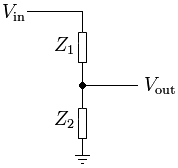
\includegraphics[width=90px,keepaspectratio]{images/Impedance_Voltage_divider.png}
                \label{fig:voltage_divider_image}
            \end{figure}
            \[ V_{out} = \frac{Z_2}{Z_1 + Z_2} V_{in} \]

        \item Capacitors, Inductors, and Resistors

            \begin{table}[h]
                \centering
                \begin{tabular}{ | l || l | l | l | l | }
                    \hline
                    Name & Voltage ($v(t)$) & Current ($i(t)$) & Laplace & Z-domain \\ \hline \hline

                    Capacitor & $v(t)$ & $C \frac{dv}{dt}$ & $sV(s) = I(s)$ & $Z_c = \frac{1}{sC}$\\ \hline
                    Inductor & $L \frac{di}{dt}$ & $i(t)$ & $V(s) = sI(s)$ & $Z_L = sL$\\ \hline
                    Resistor & $IR$ & $\frac{V}{R}$ & $V(s) = RI(s)$ & $Z_r = R$\\ \hline
                \end{tabular}
            \end{table}

        \item Ideal Op-Amps:

            \begin{figure}[h]
                \centering
                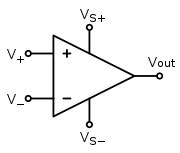
\includegraphics[width=90px,keepaspectratio]{images/180px-Op-amp_symbol.png}
            \end{figure}

            \begin{align*} V_+ = V_- \end{align*}
            \begin{align*} I_{out} = \text{arbitrary?} \end{align*}
            \begin{align*} I_+ = I_- = 0 \end{align*}

    \end{itemize}

\section{Math Review}

    \begin{itemize}
        \item Suprema:

            The maxima of an infinitely long set of elements.

        \item Convolution

            \begin{align*} f(t) * g(t) = \int_0^t {g(t-\tau) f(\tau) d\tau} = \int_0^t {f(t-\tau) g(\tau) d\tau} \end{align*}
            \begin{align*} = \Lapm^{-1}\{ G(s)F(s) \} = \Lapm^{-1}\{ F(s)G(s) \} \end{align*}

        \item Matrix Multiplication:

            \begin{align*} \left[ \begin{array}{cc} a & b \\ c & d \end{array} \right] \left[ \begin{array}{c} x \\ y \end{array} \right] = \left[ \begin{array}{c} ax + by \\ cx + dy \end{array} \right] \end{align*}

        \item Matrix Inverse:

            \begin{align*} M = \left[ \begin{array}{cc} a & b \\ c & d \end{array} \right] \end{align*}
            \begin{align*} \Rightarrow M^{-1} =  \frac{1}{det(M)} \left[ \begin{array}{cc} d & -b \\ -c & a \end{array} \right]  \end{align*}

        \item Taylor series of $f(n)$:

            Note: $f^{(n)}(a)$ is the $n^{th}$ derivative of $f$ at the point $a$.
            \begin{align*} f(x) = \Sigma_{n=0}^{\infty} \frac{f^{(n)}(a)}{n!} (x-a)^n\end{align*}

        \item Jacobians:

            If we have a function $F : \mathbbold{R}^n \to \mathbbold{R}^m$, then we have the Jacobian matrix $J$ of $F$:

            \begin{align*}
                \frac{\partial{F}}{\partial{X}}=\begin{bmatrix} \dfrac{\partial F_1}{\partial x_1} & \cdots & \dfrac{\partial F_1}{\partial x_n} \\ \vdots & \ddots & \vdots \\ \dfrac{\partial F_m}{\partial x_1} & \cdots & \dfrac{\partial F_m}{\partial x_n}  \end{bmatrix}
            \end{align*}

            i.e.
            \begin{align*}
                 \dfrac{\partial f}{\partial y}
                = \begin{bmatrix} \dfrac{\partial y_1}{\partial x_1} & \dfrac{\partial y_1}{\partial x_2} \\ \dfrac{\partial y_2}{\partial x_1} & \dfrac{\partial y_2}{\partial x_2} \\ \end{bmatrix}
            \end{align*}

        \item Laplace (\Lap):

            \begin{enumerate}
                \item $ \Lapm\{ f+g \} = \Lapm\{ f \} + \Lapm\{ g \}$
                \item $ \Lapm\{ af \} = a\Lapm\{ f \}$
                \item $ \Lapm\{ \frac{df}{dt} \} = s\Lapm\{ f \} - f'(0)$
                \item $ \Lapm\{ f*g \} = \Lapm\{ f \} \Lapm\{ g \}$
                \item $ \Lapm\{ \int_{0}^{t}f( \tau )d \tau \} = \frac{1}{s}\Lapm\{ f \}$
                \item If $ \lim_{t \to \infty} f(t) $ exists and is finite, then $\lim_{t \to \infty} f(t) = \lim_{s \to 0} sF(s)$
            \end{enumerate}

        \item Imaginary numbers and phasors: ($z \in \mathbbold{C}$)

            \begin{enumerate}
                \item $ z = x + jy \Rightarrow |z| = \sqrt{x^2 + y^2}$
                \item $ z = |z|e^{j\phase{z}} $
                \item $ z = |z| \cos(\phase{z}) + j|z|\sin(\phase{z}) $
                \item $cos(\omega t) = \frac{e^{j\omega t} + e^{-j\omega t}}{2} $
                \item $sin(\omega t) = \frac{e^{j\omega t} - e^{-j\omega t}}{2j} $
                \item $\phase{\frac{ab}{c}} = \phase{a} + \phase{b} - \phase{c}$
            \end{enumerate}

        \item Log Laws:

            \begin{enumerate}
                \item $\log(\left|\frac{ab}{c}\right|) = \log(|a|) + \log(|b|) - \log(|c|)$
            \end{enumerate}

        \item Identifying 1st vs 2nd Order ODEs:

            ($k, \tau, \omega_n$ are constants)

            \begin{itemize}
                \item 1st order:

                    \begin{align*}
                        \tau \dy + y = Ku &\Rightarrow^{\Lapm} G(s) = \frac{K}{1+s\tau} \\
                        &\text{or} \\
                        \dx &= \frac{-x}{\tau} + \frac{Ku}{\tau} \\ y &= x
                    \end{align*}

                \item 2nd order:

                    \begin{align*}
                        \ddy + 2\zeta \omega_n \dy + \omega_n^2 y = K\omega_n^2u &\Rightarrow^{\Lapm} G(s) = \frac{K \omega_n^2}{s^2 + 2s\omega_n \zeta + \omega_n^2} \\
                        &\text{or} \\
                        \dx_1 &= x_2 \\ \dx_2 &= -\omega_n^2 -2 \zeta \omega_n x_2 + K \omega_n^2 u \\ y &= x_1 \\
                    \end{align*}
            \end{itemize}
        \item Z-transform:

            $Z^{-1}$ corresponds to going back in time.
    \end{itemize}

\section{Physics Review}

    \begin{itemize}
        \item Newton's 2nd Law

            \begin{align*} M \ddy = F \end{align*}
            \begin{align*} \Sigma F  = M \ddy \end{align*}

    \end{itemize}

\end{document}
